%%%%%%%%%%%%%%%%%%%%%%%%%%%%%%%%%%%%%%%%%%%%%%%%%%%%%%%%%%%%%%%%%%%%%%
%% The class has several options, the default is oneside, onecolumn, 10pt, final
%
%  onecolumn/twocolumn - format for one or two columns per page
%  10pt/11pt/12pt - use 10, 11, or 12 point font
%  oneside/twoside - format for neside/twosided printing
%  final/draft - format for final/draft copy
%  cleanfoot - take out copyright info in footer leave page number
%  cleanhead - take out the conference banner on the title page
%  titlepage/notitlepage - put in titlepage or leave out titlepage

\documentclass[twocolumn,10pt]{asme2e}
\usepackage{graphicx}
\usepackage{epstopdf}
\usepackage{dblfloatfix}
\usepackage{cite}
\special{papersize=8.5in,11in}


%%%%%%%%%%%%%%%%%%%%%%%%%%%%%%%%%%%%%%%%%%%%%%%%%%%%%%%%%%%%%%%%%%%%%%
\confshortname{OMAE2015}
\conffullname{ASME the 2015 34th International Conference on Ocean, Offshore and Arctic Engineering}

%% for date in a single month, use
%\confdate{24-28}
%\confmonth{September}
%% for date across two months, use
\confdate{May 31-June 5}
\confyear{2015}
\confcity{St. John's, NL}
\confcountry{Canada}


\papernum{OMAE2015-42074}

%%%%%%%%%%%%%%%%%%%%%%%%%%%%%%%%%%%%%%%%%%%%%%%%%%%%%%%%%%%%%%%%%%%%%%
% Title
% You need to remove 'DRAFT: ' in the title for the final submitted version.

\title{Development of PTO-Sim: a power performance module for the open-source wave energy converter code WEC-Sim}


%%%%%%%%%%%%%%%%%%%%%%%%%%%%%%%%%%%%%%%%%%%%%%%%%%%%%%%%%%%%%%%%%%%%%%
% Authors

% osu authors
\author{Ratanak So\\
       {\tensfb Asher Simmons}   \\
       {\tensfb Ted Brekken}   
    \affiliation{
	School of Electrical Engineering and Computer Science\\
	Oregon State University\\
	Corvallis, Oregon USA\\
    }	
}

% snl authors
\author{Kelley Ruehl \thanks{Address all correspondence to this author.} \\
       {\tensfb Carlos Michelen}     
    \affiliation{Water Power Department \\
    	Sandia National Laboratories\\
	Albuquerque, NM USA\\
	Email: kelley.ruehl@sandia.gov
    }
}


\begin{document}
\maketitle    


%%%%%%%%%%%%%%%%%%%%%%%%%%%%%%%%%%%%%%%%%%%%%%%%%%%%%%%%%%%%%%%%%%%%%%
\begin{abstract}
{\it 
WEC-Sim (Wave Energy Converter-SIMulator) is an open-source wave energy converter (WEC) code capable of simulating WECs of arbitrary device geometry subject to operational waves. The code is developed in MATLAB/Simulink using the multi-body dynamics solver SimMechanics, and relies on Boundary Element Method (BEM) codes to obtain hydrodynamic coefficients such as added mass, radiation damping, and wave excitation. WEC-Sim Version 1.0, released in Summer 2014, models WECs as a combination of rigid bodies, joints, linear power take-offs (PTOs), and mooring systems. This paper outlines the development of PTO-Sim (Power Take Off-SIMulator), the WEC-Sim module responsible for accurately modeling a WEC's conversion of mechanical power to electrical power through its PTO system. PTO-Sim consists of a Simulink library of PTO component blocks that can be linked together to model different PTO systems. Two different applications of PTO-Sim will be given in this paper: a hydraulic power take-off system model, and a direct drive power take-off system model.
}
\end{abstract}


%%%%%%%%%%%%%%%%%%%%%%%%%%%%%%%%%%%%%%%%%%%%%%%%%%%%%%%%%%%%%%%%%%%%%%
\section*{INTRODUCTION}

Sandia National Laboratories (SNL) and the National Renewable Energy Laboratory (NREL) have jointly developed WEC-Sim (Wave Energy Converter-SIMulator), an open-source wave energy converter (WEC) design tool capable of running on a standard personal computer. WEC-Sim  simulates WECs of arbitrary device geometry subject to operational waves \cite{wecsim}. The code is developed in MATLAB/Simulink using the multi-body dynamics solver SimMechanics, and relies on Boundary Element Method (BEM) codes to obtain hydrodynamic coefficients such as added mass, radiation damping, and wave excitation. The WEC-Sim hydrodynamic solution has been verified through code-to-code comparison, and has undergone preliminary validation through comparison to experimental data \cite{yu2014design}\cite{lawson2014implementing} \cite{ruehl2014preliminary}\cite{yu2014development}.  
Further validation of the WEC-Sim code will be performed upon completion of the WEC-Sim validation tank testing, scheduled for Summer 2015. 

Version 1.0 of WEC-Sim, released in Summer 2014, models WECs as a combination of rigid bodies, joints, linear power take-offs (PTOs), and mooring systems. While the Version 1.0 release of the WEC-Sim code was limited to modeling PTOs as simple linear dampers, collaboration with the Energy Systems group at Oregon State University (OSU) has resulted in the development of PTO-Sim (Power Take Off-SIMulator). PTO-Sim is the WEC-Sim module responsible for accurately modeling a WEC's conversion of mechanical power to electrical power through its PTO system (or power conversion chain, PCC). It consists of a library of PTO component blocks that can be linked together to model different PTO systems. Each of these PTO library blocks is a model of common PTO components, such as electric generators, pistons, and accumulators. Two different applications of PTO-Sim will be given in this paper: a hydraulic power take-off system model, and  a linear direct drive power take-off system model. 


%%%%%%%%%%%%%%%%%%%%%%%%%%%%%%%%%%%%%%%%%%%%%%%%%%%%%%%%%%%%%%%%%%%%%%
\section*{POWER CONVERSION CHAINS}

% TB: Double column floats get put after the page they are instantiated in, so I put it at the beginning to get it to appear on the next page where it fit better
\begin{figure*}[t] 
    \centering
    %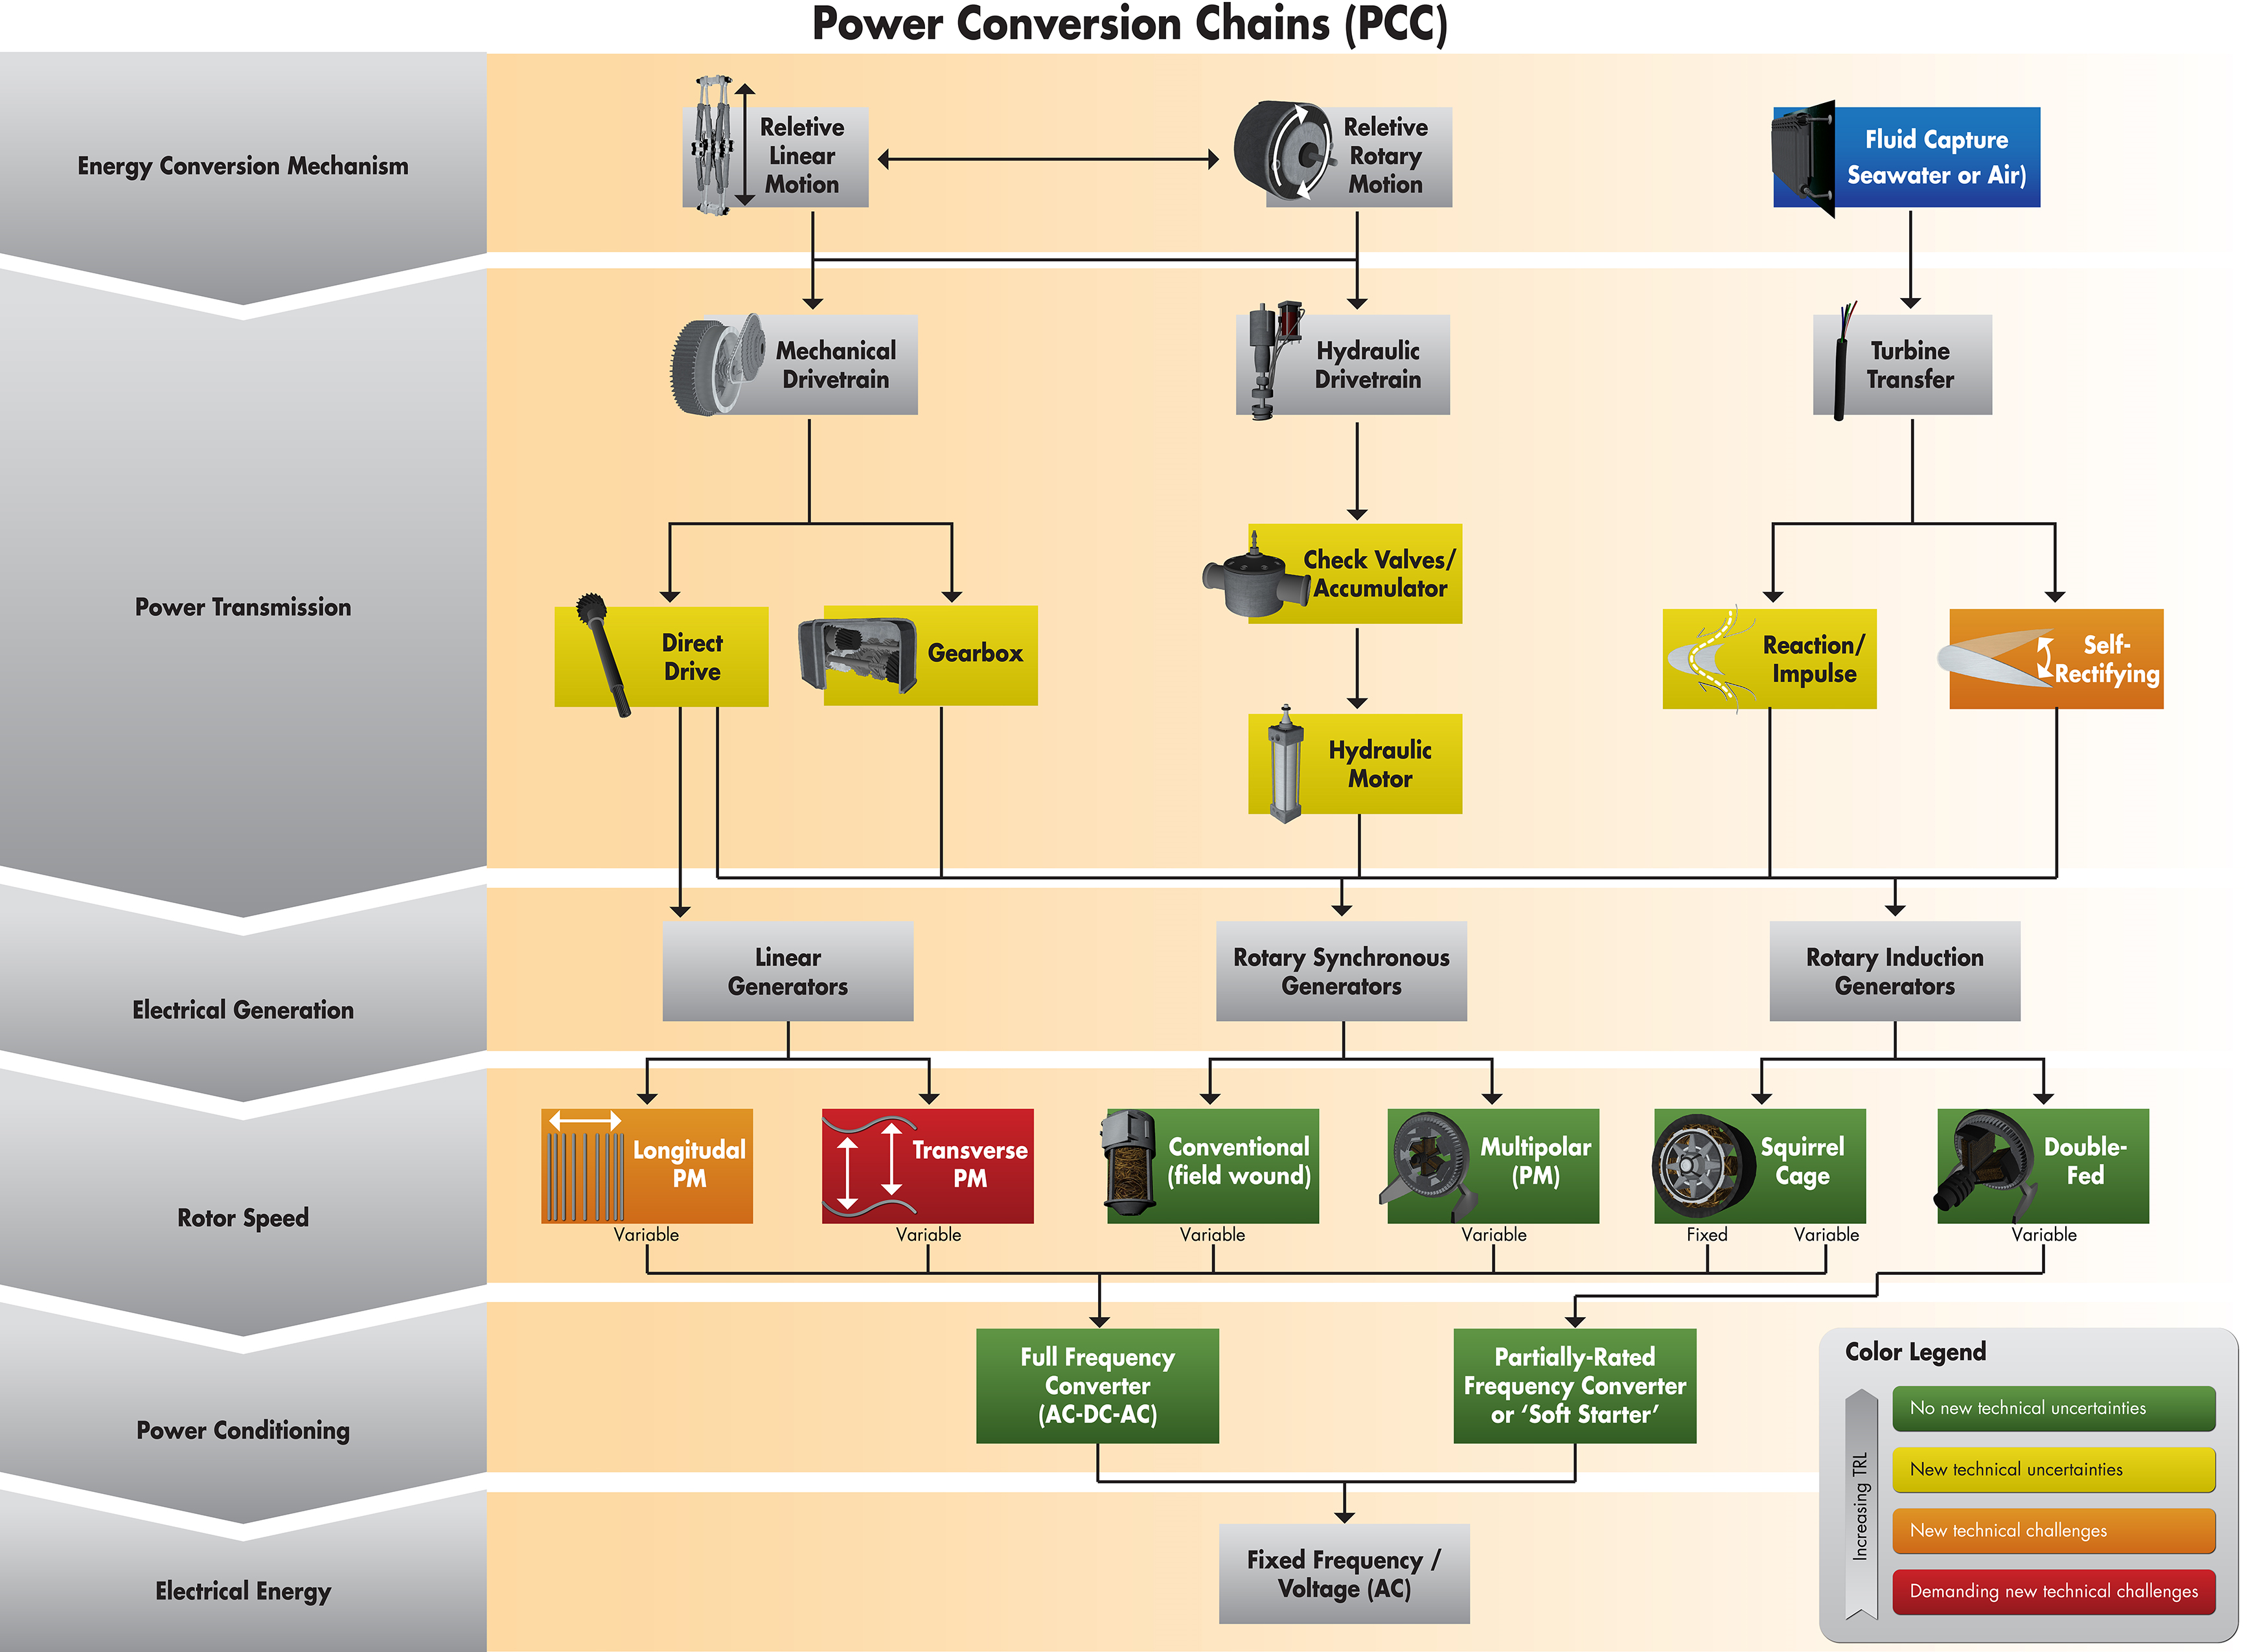
\includegraphics[width=1.95\columnwidth]{Images/PCC}
    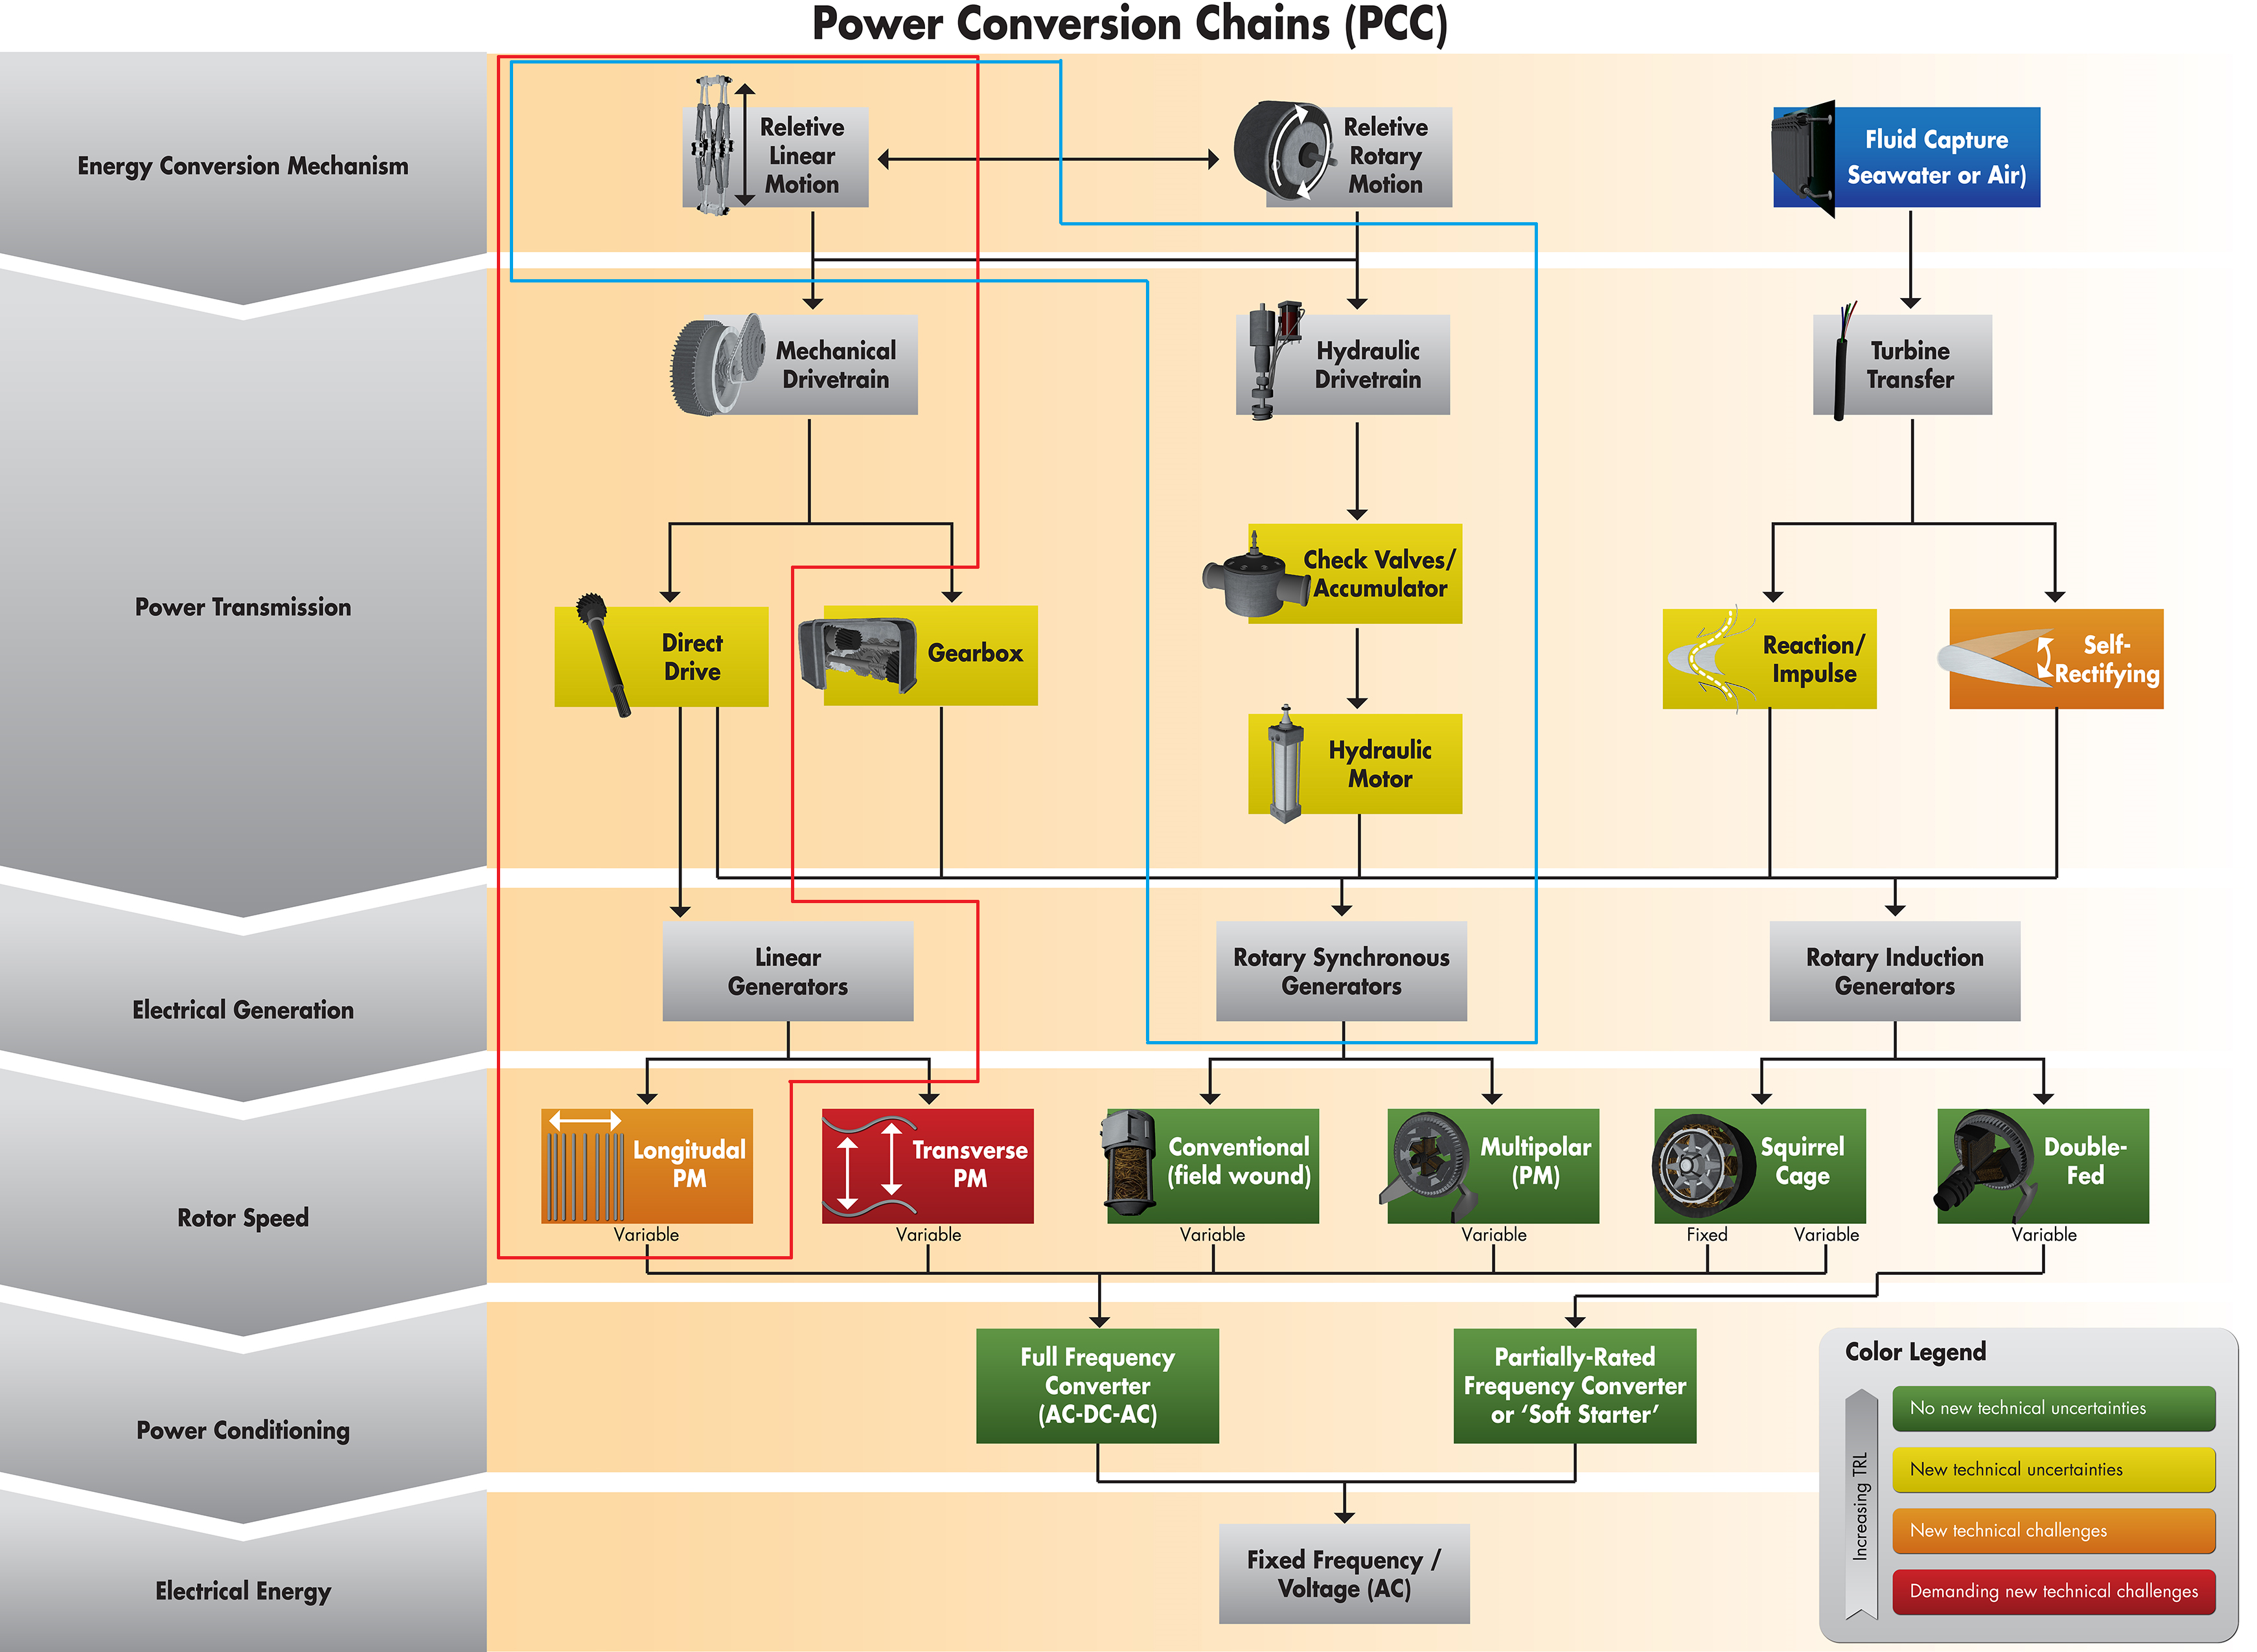
\includegraphics[width=1.95\columnwidth]{Images/PCC_HydDD}
    \caption{Power conversion chain from mechanical energy to electrical connection to grid. Lower TRLs are novel concepts and higher TRLs are more proven technology. The direct drive PTO path is shown in the red box outline and the hydraulic PTO path is shown in the blue box outline.}
    \label{PCC}
    \end{figure*}

\begin{figure}[t]
    \centering
    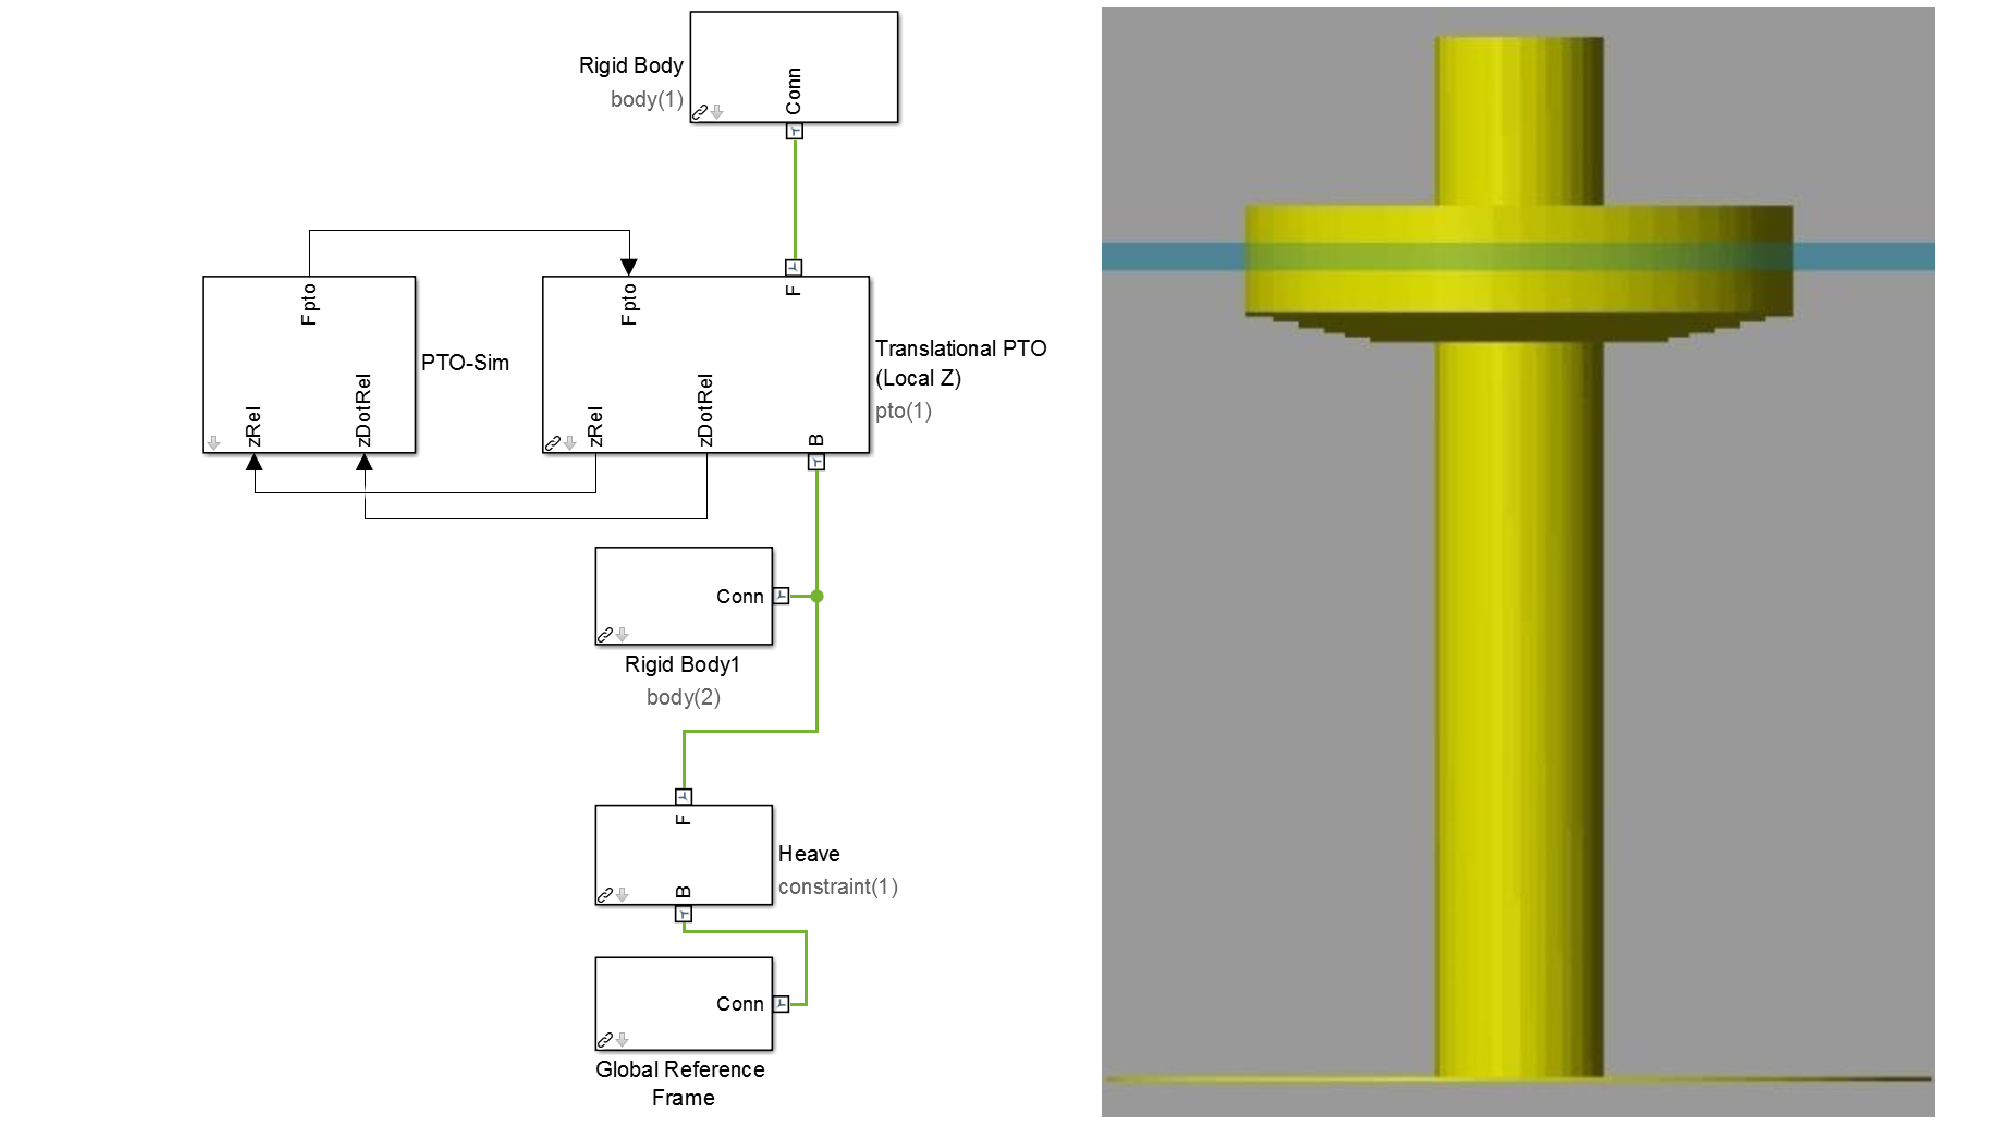
\includegraphics[width=1\columnwidth]{Images/RM3_update}
    \caption{RM3 model with PTO-Sim (left) with the animation (right) [1].}
    \label{RM3}
    \end{figure}

\begin{figure}[t]
    \centering
    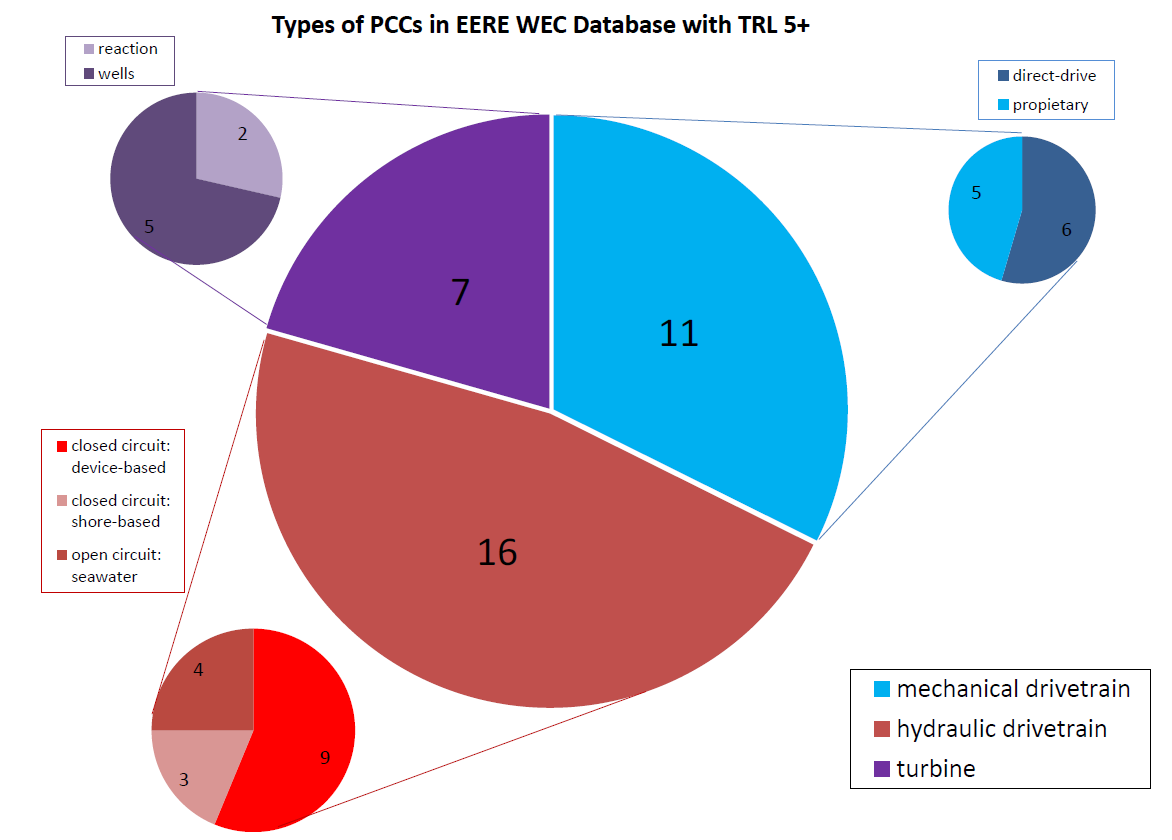
\includegraphics[width=1\columnwidth]{Images/TRL}
    \caption{Breakdown of PCC types currently used by companies with TRL equal to or greater than 5.}
    \label{PCC_Breakdown}
    \end{figure}

%Note (Kelley): I decided not to do a PTO background section as previously intended because it didn't seem necessary. If we change our mind, I can add it for the final submission

A WEC's power conversion chain converts the mechanical motion of the WEC into electrical power. The majority of WECs convert the energy from the wave into either relative linear motion, relative rotary motion, or fluid capture. This mechanical power is then converted into electrical power through the WEC's PCC. There are many different possible PCC configurations, as shown in Fig~\ref{PCC}. On the left side of the figure is the energy conversion mechanism, and on the right side are different PCC components with black arrows indicate possible PCC paths. The Color Legend refers to technological readiness level of each PCC component \cite{reed2010accelerating}\cite{ruehl2012wave}. This technological readiness level is based on the work in the DNV Recommended Practices which takes into consideration both the degree of the novelty of the technology and its intended application \cite{veritas2001recommended}. 

Based on a survey of the EERE WEC database, there are 34 WEC PCCs that are at a technology readiness level (TRL) 5 or greater \cite{eere}. Of these 34 WEC PCCs, 16 use a hydraulic PTO, 11 use a mechanical PTO, and 7 use a turbine, see Fig.~\ref{PCC_Breakdown}. Of the 11 mechanical PTOs, 6 are direct drive systems. The results of this survey, and current trends in the WEC industry, drove the development of hydraulic and direct drive application cases PTO-Sim. These two application cases will be released with future versions of the WEC-Sim code. Since WEC-Sim is an open source code, and there are many different possible PCC configurations, users can create PCC specific models to meet their needs. These can be built based on existing PTO-Sim library blocks, or by creating new PCC component blocks.


%%%%%%%%%%%%%%%%%%%%%%%%%%%%%%%%%%%%%%%%%%%%%%%%%%%%%%%%%%%%%%%%%%%%%%
\section*{PTO-SIM}

WEC-Sim consists of a library of different WEC components, namely: bodies, joints and constraints. These WEC-Sim library blocks can be linked together to model the hydrodynamic behavior of different WEC devices. An example of applying the WEC-Sim code to model the Reference Model 3 (RM3) point absorber is shown Fig.~\ref{RM3}. The RM3 was designed as part of the DOE-funded Reference Model Project \cite{sandia}. RM3 is a simple two-body point absorber, consisting of a float and a damping plate. The float is connected to the damping plate through a translational joint which is actuated by the external PTO-Sim subsystem that simulates the PTO system. The damping plate is then connected to the seabed through a 3 degrees of freedom (DOF) (SimMechanics planar joint) floating connection (accounting for the mooring system). This paper specifically focuses on what is inside the PTO-Sim block on the left side of Fig.~\ref{RM3}.

PTO-Sim is developed in a similar manner to WEC-Sim, as a library of different PCC components. The PTO-Sim library has been developed based on the possible PCC configurations outlined in Fig~\ref{PCC}. In the following sections, the PTO-Sim component library will be used to model a hydraulic PTO, and a direct drive PTO. For purposes of describing PTO-Sim operation, as shown in Fig.~\ref{RM3}, the WEC-Sim outputs (zRel) and (zDotRel) are the PTO-Sim inputs, and the WEC-Sim input (Fpto) is the PTO-Sim output for both PTO architectures demonstrated in this paper.  These signals are what couple WEC-Sim and PTO-Sim together, as shown in Fig.~\ref{RM3}. Most WEC PCCs are complex and device specific, meaning that while some WEC PTO models can be build from the PTO-Sim library, many while require custom PCC library components. 

It should be noted that the WEC-Sim is fully coupled with PTO-Sim. 

%Note (Kelley): Include an image of the WEC-Sim and PTO-Sim libraries for reference in this section

%Note (Kelley): Add reference to IEEE paper for Final submission (not this one)


%%%%%%%%%%%%%%%%%%%%%%%%%%%%%%%%%%%%%%%%%%%%%%%%%%%%%%%%%%%%%%%%%%%%%%
\subsection*{Hydraulic PTO}
An example of a hydraulic PTO used in a point absorber is shown in Fig. 4.  The piston position and velocity are the relative position and velocity between the float and the spar. The first PTO system element is a double acting hydraulic piston pump, ``P". This component directly converts the heave motion of the buoy into a pressurized, bi-directional fluid flow. The piston chamber is connected to a rectifying valve via terminals ``A" and ``B". This changes the bi-directional flow into a uni-directional flow and passes the fluid on to the rest of the system. The valves ``1" through ``4" indicate the different flow paths that perform this conversion. Valve ``1" delivers fluid to the high pressure side of the system where it is stored in the high pressure accumulator ``C". A variable displacement motor, ``M", translates the hydraulic fluid power into rotational energy. The axle of the motor is connected directly (no gearboxes) to a generator (``G") axle, causing it to spin and generate electricity. The hydraulic motor was chosen to meet the torque and speed requirements. The maximum speed the motor can spin is 2400 rpm.
The hydraulic fluid then enters the low pressure side where accumulator ``D" provides pressure control. The piston draws fluid from ``D", completing the circuit \cite{casey2013modeling}.

\begin{figure}[t]
    \centering
    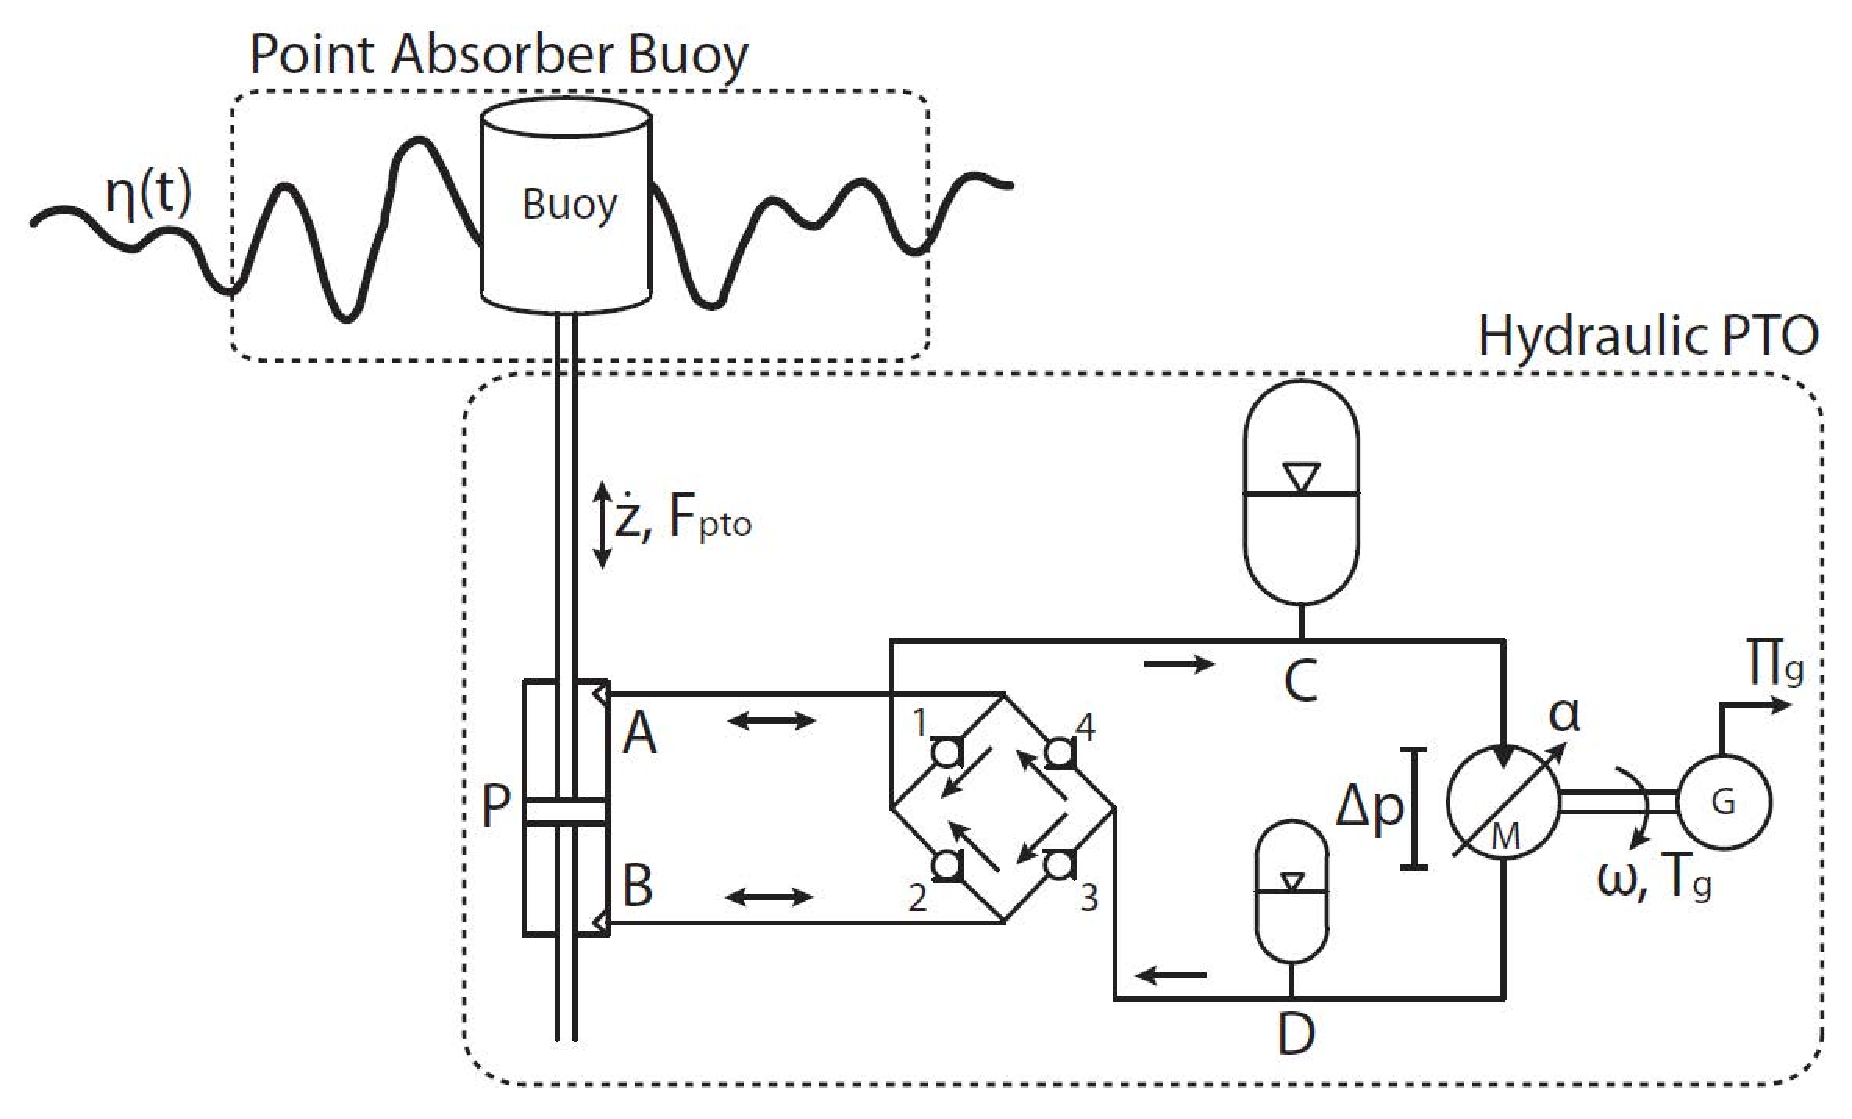
\includegraphics[width=1\columnwidth]{Images/HydraulicPTO}
    \caption{Schematic of the PTO-Sim hydraulic model. The arrow indicate the direction of flow.}
    \label{HydPTO}
    \end{figure}

The hydraulic PTO model begins with the continuity equation for a compressible fluid, which is used to describe the pressures in the piston chamber \cite{merritthydraulic}:

\begin{equation}
\dot{p}_A=\frac{\beta_e}{V_o-A_pz}(A_p\dot{z}-\dot{V_1}+\dot{V_4}) 
\end{equation}
\begin{equation}
\dot{p}_B=\frac{\beta_e}{V_o+A_pz}(-A_p\dot{z}-\dot{V_2}+\dot{V_3}) 
\end{equation}

The effective bulk modulus of the hydraulic fluid is $\beta_e$, $V_o$ is the initial volume of the cylinder, and $A_p$ is the piston area. The volumetric flows through valves 1-4 are represented by $\dot{V}_1$ through $\dot{V}_4$. The piston and buoy are rigidly connected, and their movement with respect to the spar is the input to the 
PTO system. This relative movement is the velocity of $\dot{z}$.

The four valves in the rectifying circuit are each modeled using the orifice equation: 

\begin{equation}
\dot{V}_i=C_dA_v \sqrt{\frac{2}{\rho}(p_j-p_k)\tanh(k_1(p_j-p_k))}  
\end{equation}

The subscript ``$i$" refers to the valve number. $C_d$ is the discharge coefficient and $A_v$ is the cross-section area of the orifice. Finally, $p_j$ and $p_k$ are the pressures on either side of the valve. The $tanh$ function, being differentiable, enables certain  control/optimization strategies as well as simplifying
the calculations. 

The valve area is modeled as a variable area poppet valve, with the equation:  

\begin{eqnarray}
A_v &=& A_{min}+\frac{A_{max}-A_{min}}{2}+\nonumber\\
&& \frac{A_{max}-A_{min}}{2}(\tanh(k_2(p_j-p_k-\frac{p_{max}+p_{min}}{2})))
\end{eqnarray}

\noindent where $A_{max}$ and $A_{min}$ are the maximum and minimum valve areas. The valve begins to open when $p_{min}$ is reached. The maximum pressure, $p_{max}$ is the pressure for which the valve is fully opened.  The $tanh$ function in this equation provides a smooth approximation to the step operation of the 
valve. This is accomplished by choosing $k_2$ such that when the pressure difference ($p_j$ - $p_k$) is equal to $p_{max}$, the valve area difference ($A_{v}$-$A_{min}$) is equal to $A_{min}$. The behavior of the valve is shown in Fig. 5. 

\begin{figure}[t]
    \centering
    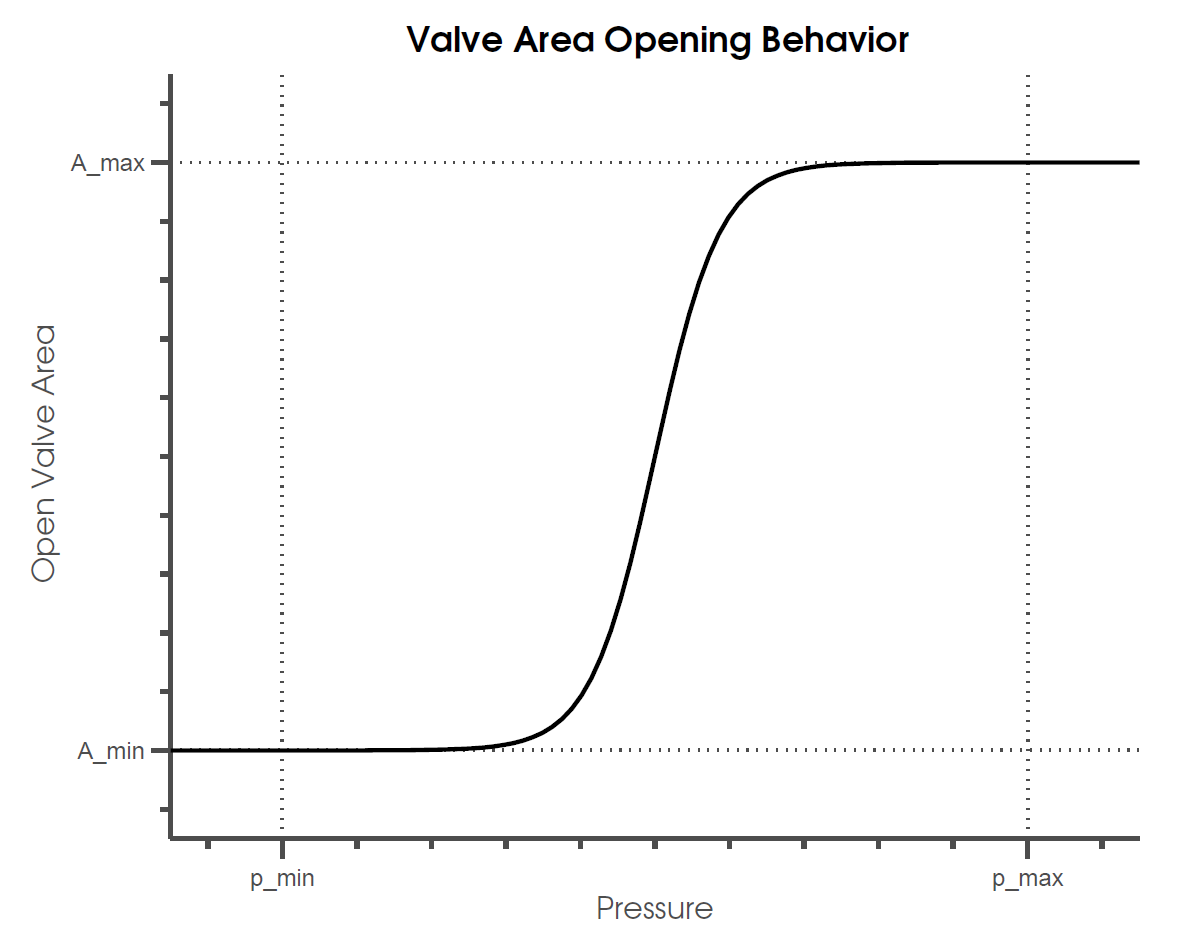
\includegraphics[width=1\columnwidth]{Images/ValveBehavior}
    \caption{Valve opening behavior as a function of pressure difference across the valve.}
    %\label{fig-freq-comparison}
    \end{figure}    

\begin{figure*}[t]	
    \centering
    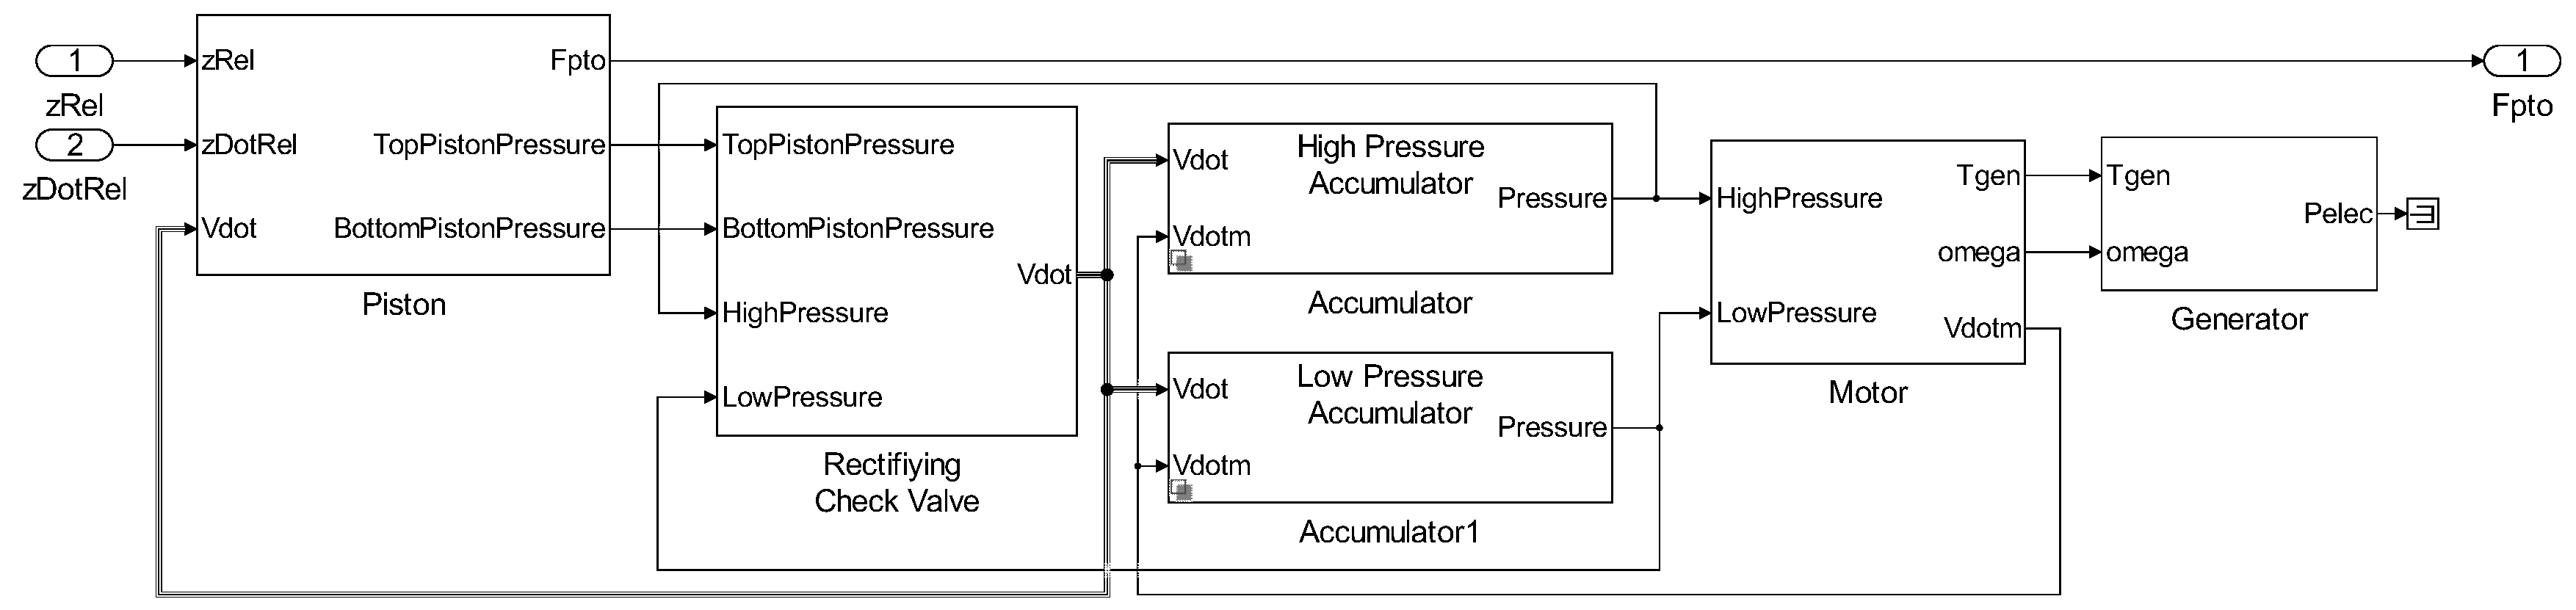
\includegraphics[width=2\columnwidth]{Images/ptomodel}  
    \caption{Simulink model of the hydraulic system.}
    \label{Hyd}
    \end{figure*}

The flow into the accumulators ``C" and ``D" are, respectively: 
\begin{equation}
\dot{V}_C=-\alpha D \omega+\dot{V}_1+\dot{V}_2 
\end{equation}

\begin{equation}
\dot{V}_D=\alpha D \omega-\dot{V}_3-\dot{V}_4 
\end{equation}

\noindent where $\alpha$ is the swashplate angle ratio, which is the instantaneous motor displacement divided by the the maximum motor displacement. It is used as a control for the volumetric flow across the motor. $D$ is the nominal motor displacement, and $\omega$ is the rotational speed of the generator. 
For this hydraulic system the swashplate angle ratio is fixed for the simulated sea state. 

The pressure in each accumulator is dependent on the instantaneous volume of hydraulic fluid in the accumulator:

\begin{equation}
p_i=\frac{p_{i0}}{(1-\frac{V_i}{V_{i0}})^{1.4}}
\end{equation}

\noindent where $p_{i0}$ is the precharge pressure and $V_{i0}$ is the total volume of the accumulator. 

Because the motor axle and generator axle are rigidly connected, they have the same torque and opposite rotational direction. This condition leads to the state equation:

\begin{equation}
\dot{\omega}=\frac{1}{J_t}(\alpha D (p_C-p_D)-b_g \omega-b_f \omega)
\end{equation}

The generator torque is represented by $b_g$$\omega$, $b_f$$\omega$ is the frictional damping, and $J_t$ is the total mass moment of inertia of the motor/generator drive train.  The frictional damping was chosen to give the generator a 95\% efficiency at a speed of 2400 rpm. 

Finally, the PTO force is described by the A-B pressure differential and the piston area under pressure, $A_p$:

\begin{equation}
F_{pto}=(p_A-p_B)A_p
\end{equation}

These equations are contained in PTO-Sim library blocks that represent physical components of the hydraulic PTO system. The complete hydraulic PTO model as implemented using PTO-Sim is shown in Fig.~\ref{Hyd}. Although hydraulic PTO may seem complex as shown in Fig. \ref{HydPTO}, it gives a much more realistic estimate of power produced. 

\subsubsection*{Simulations.}

Figures~\ref{HydZdot} and \ref{HydP} show a sample (from 500-600 seconds) of the simulation. Figure~\ref{HydZdot} shows the system inputs, ``zRel (Relative heave position) and zDotRel (relative heave velocity)". Figure~\ref{HydP} shows the power produced in the PTO. The blue line, $P_{abs}$ is the power absorbed at the piston. $P_{gen}$, the power at the axle connecting the motor and generator, is shown in red. Finally, $P_{elec}$ is the electrical power at the output of the generator, is shown in yellow. The generator model is based on the characteristics of a typical large industrial induction generator. The speed, torque, and efficiency of this motor are taken from a lookup table and used as a simple rotational inertial model. 


\begin{figure}[t]
    \centering
    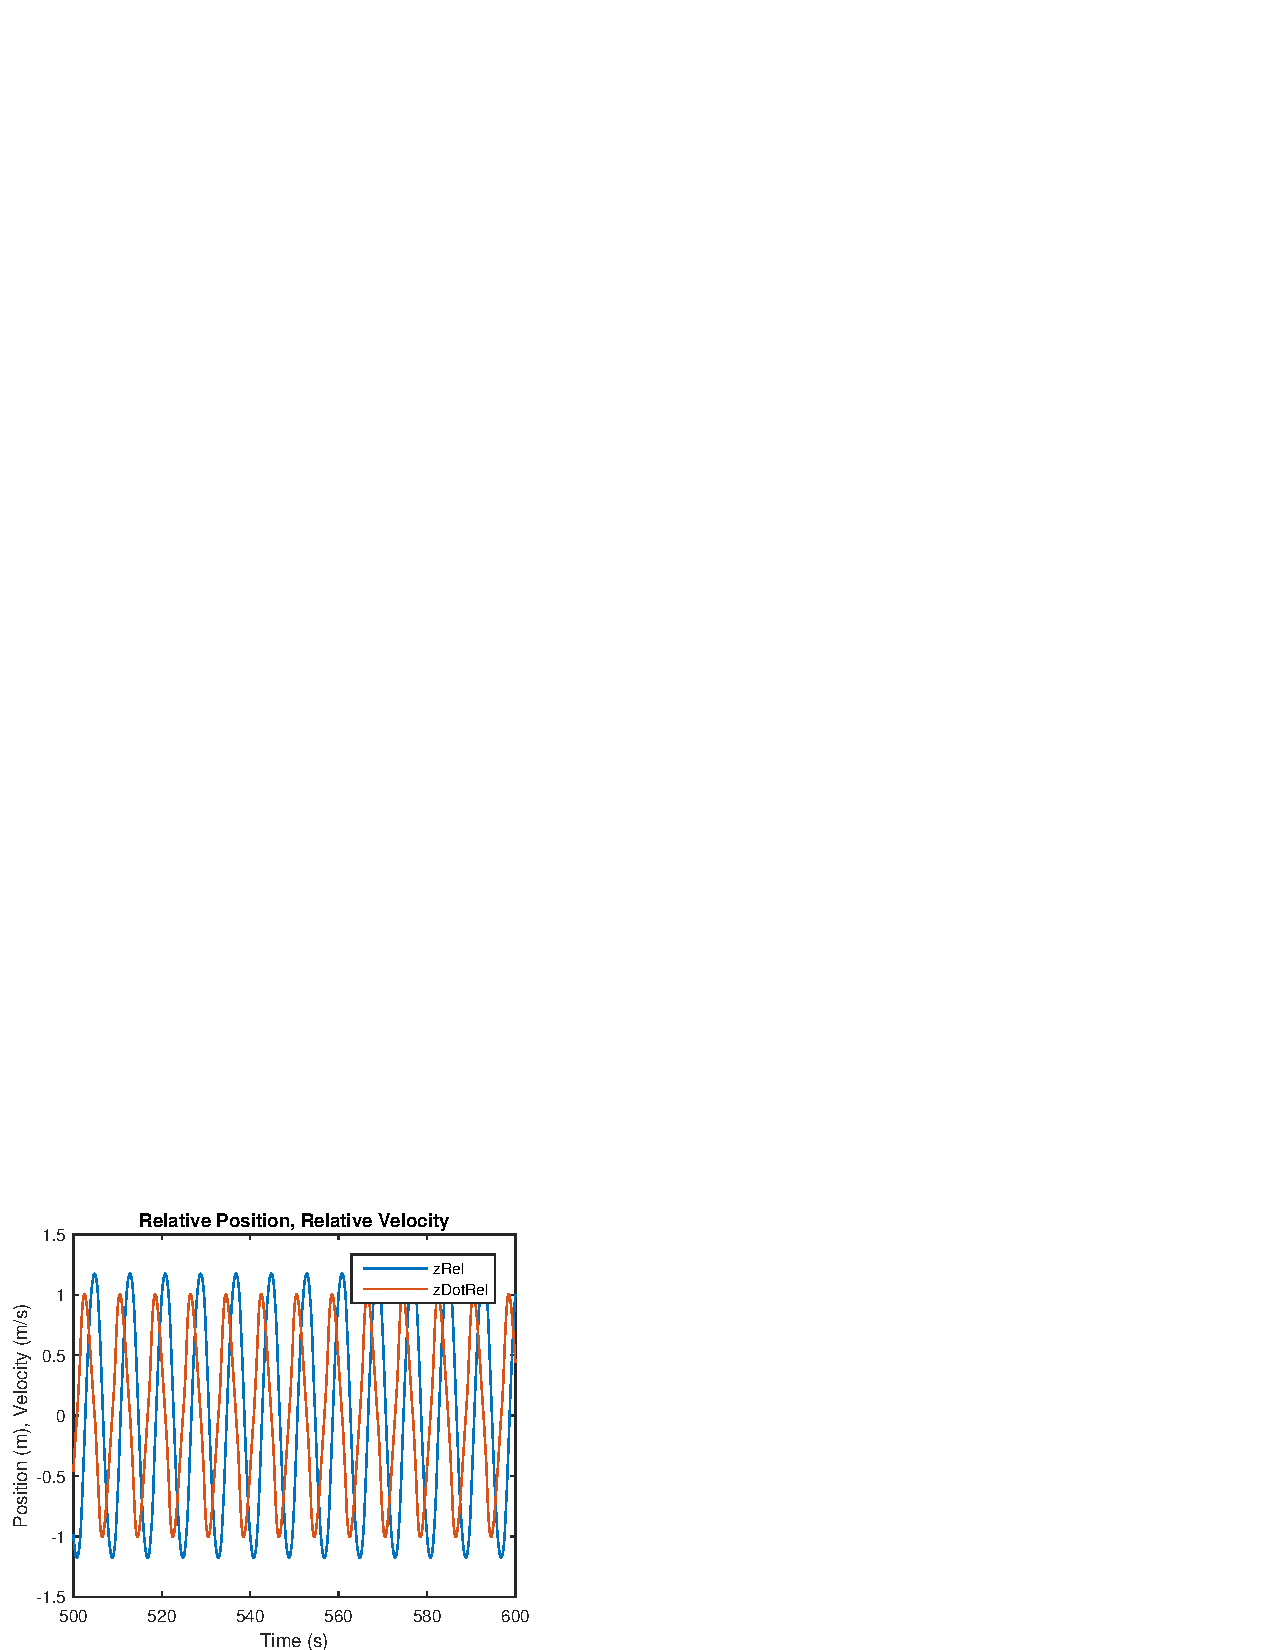
\includegraphics[width=1\columnwidth]{Images/zRelzDotRel} %DDzDot
    \caption{Relative position and velocity for a wave of 3 meters with a period of 8 seconds.}
    \label{HydZdot}
    \end{figure}

\begin{figure}[t]
    \centering
    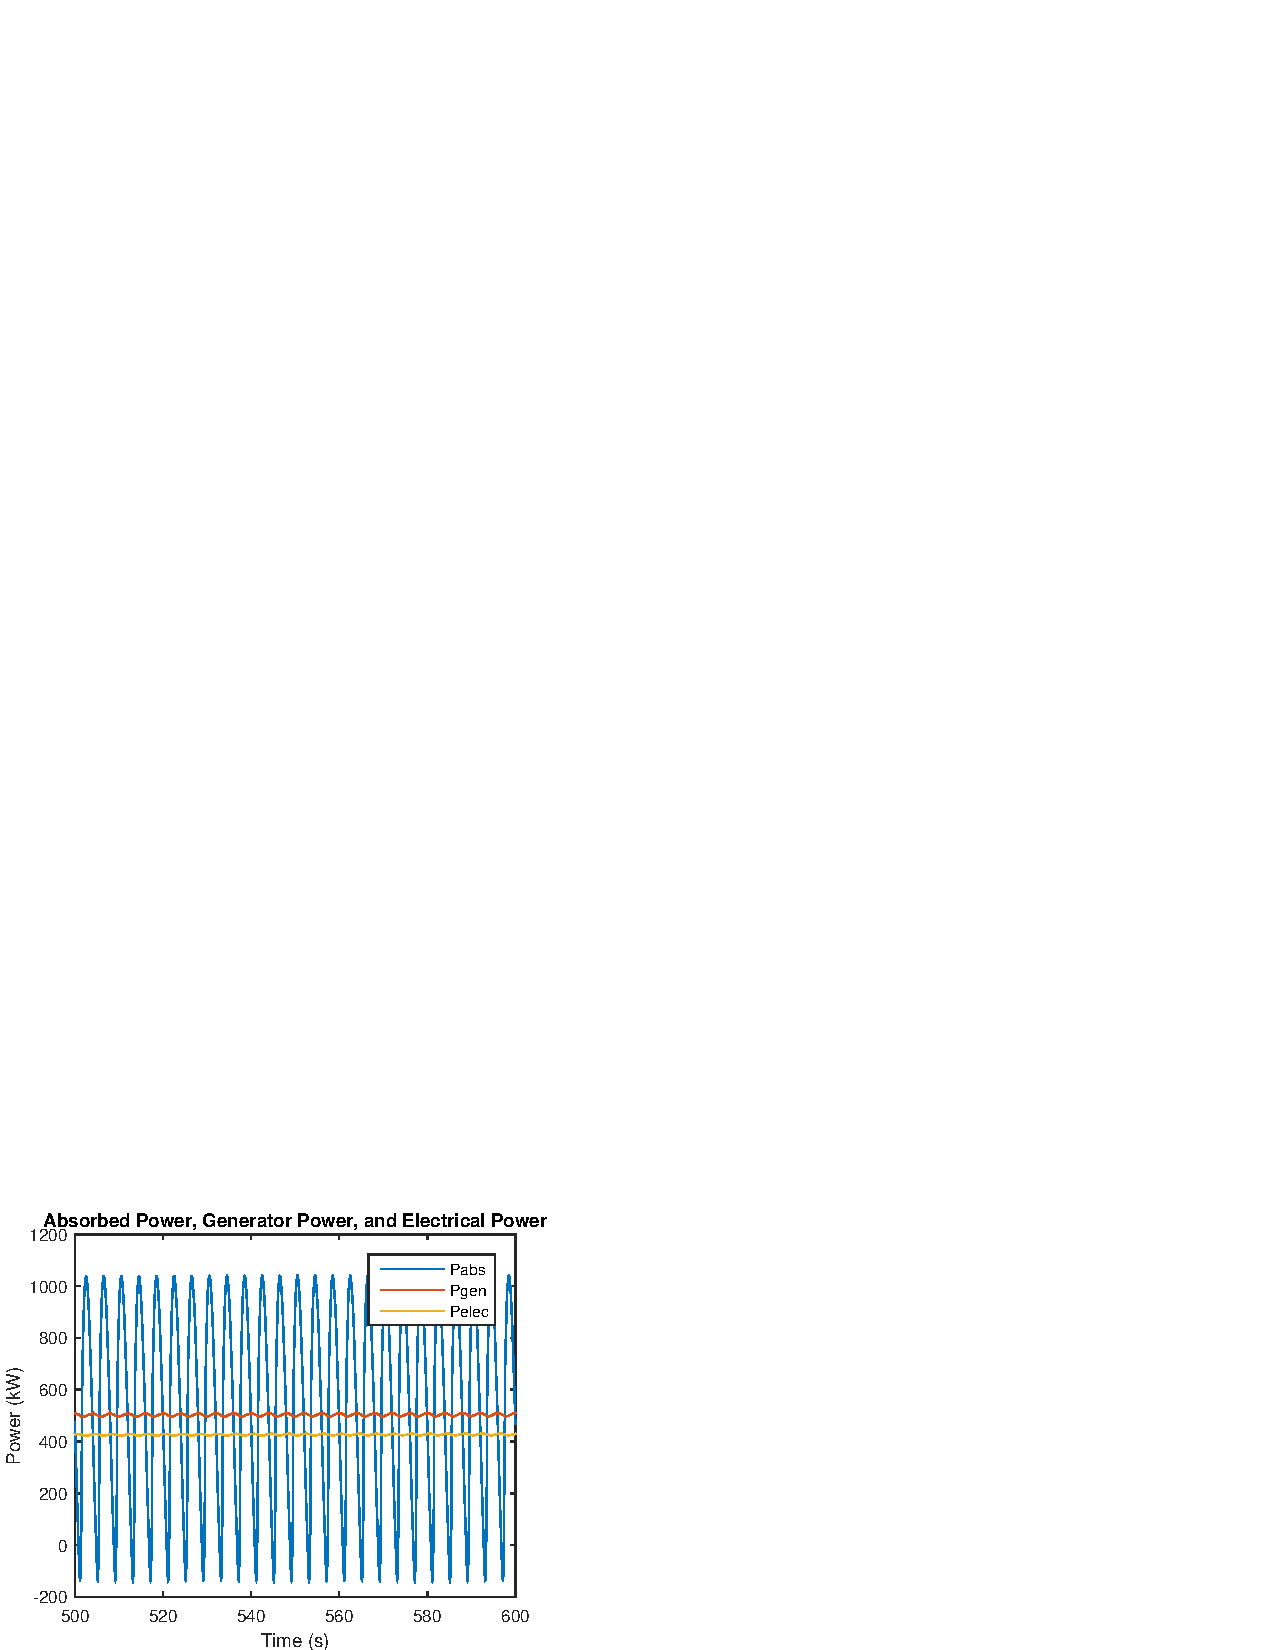
\includegraphics[width=1\columnwidth]{Images/HYDPower}
    \caption{Absorbed, mechanical, and electrical power. }
    \label{HydP}
    \end{figure}

The hydraulic power can reach negative values when the relative heave velocity is close to zero but its  average value is typically larger than the electrical power because there are some losses in the valves. A negative value presented in Fig.~\ref{HydP} means that the hydraulic PTO is releasing energy to the buoy at some instants. This event is typically related to phase control system that when the control accumulators are activated, the hydraulic PTO is therefore releasing large amount of energy to the buoy. As a result, it is due to the large volumes chosen for the high and low pressure accumulators and it has been seen that smaller accumulators would determine larger output variations \cite{yukio2014modeling}.

The system response is shown in Figs.~\ref{HydF} and~\ref{HydPr}. When the pressure exceeds $p_{min}$, the valves will open. This hydraulic system therefore manifests an intrinsic latching control \cite{falnes2005ocean}.

\begin{figure}[t]
    \centering
    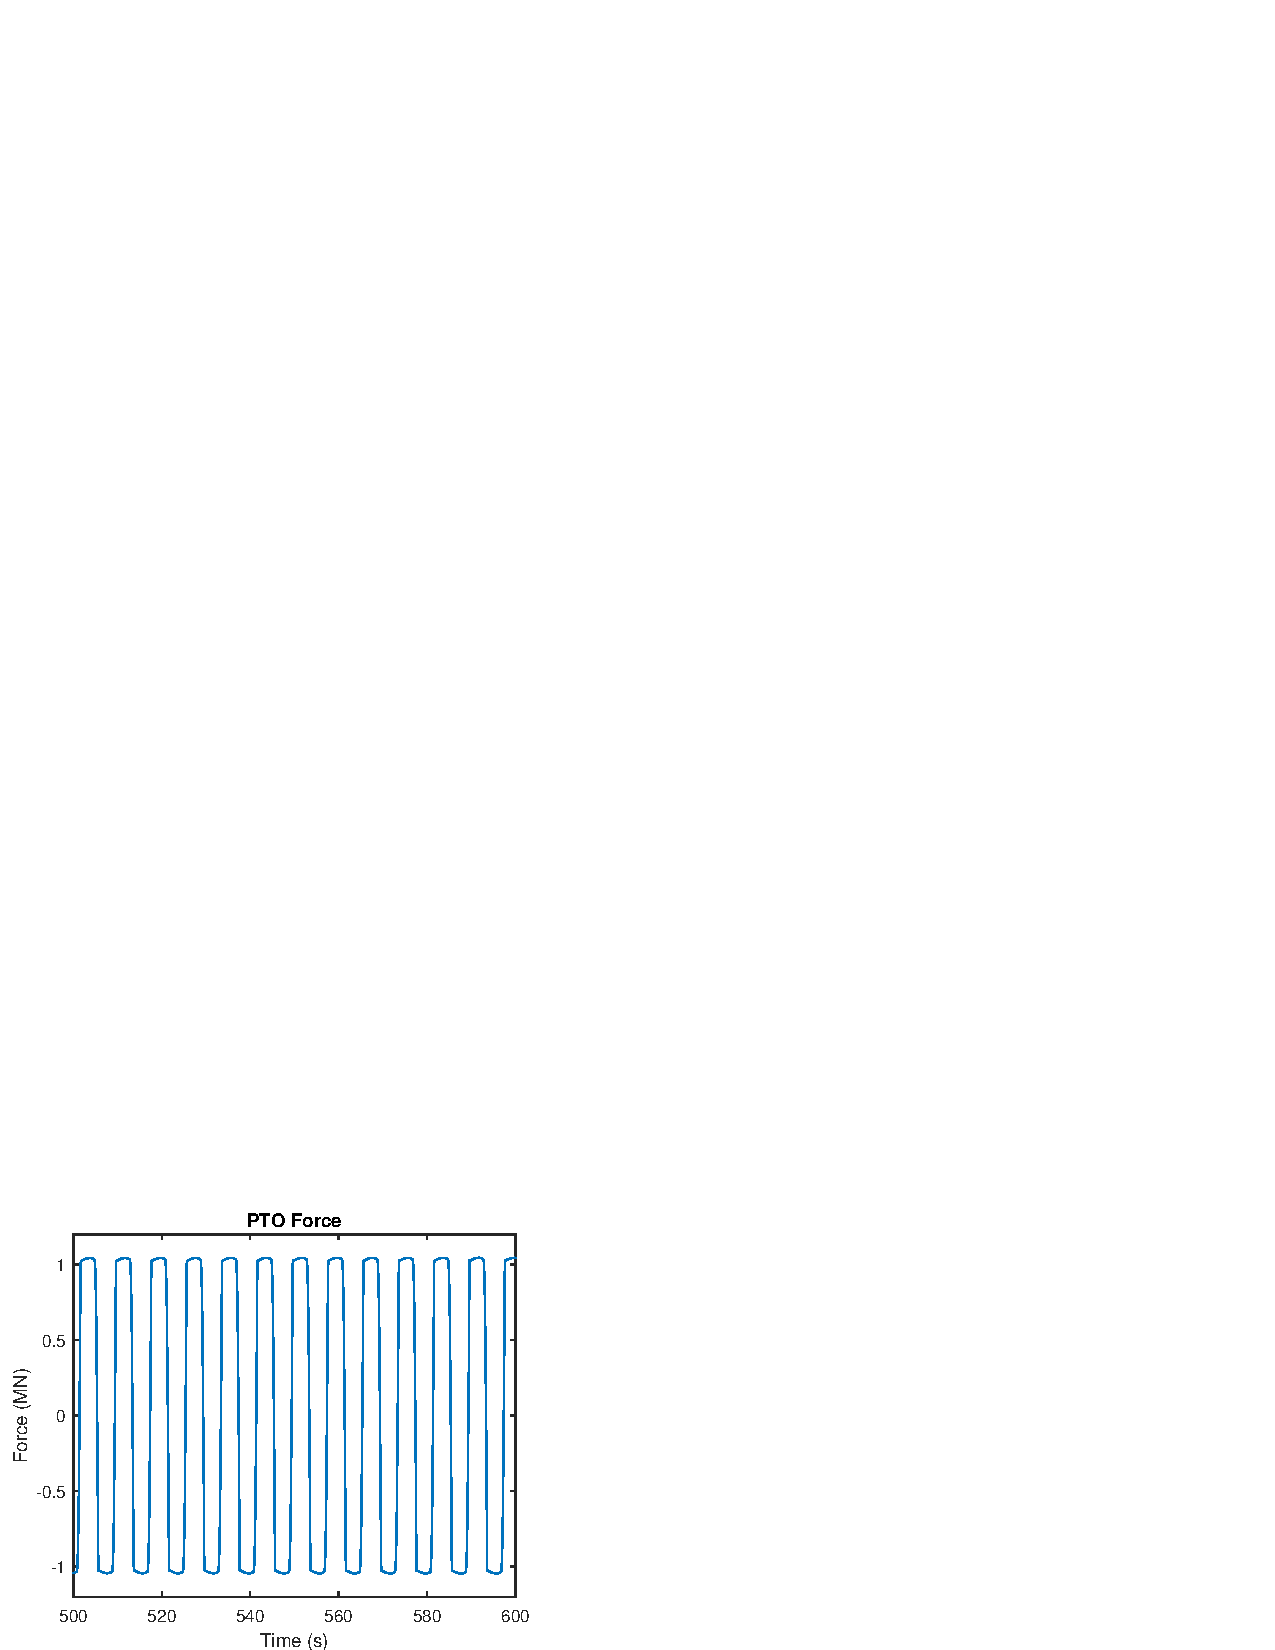
\includegraphics[width=1\columnwidth]{Images/ptoForce}
    \caption{Force applied by the PTO.}
    \label{HydF}
    \end{figure}

\begin{figure}[t]
    \centering
    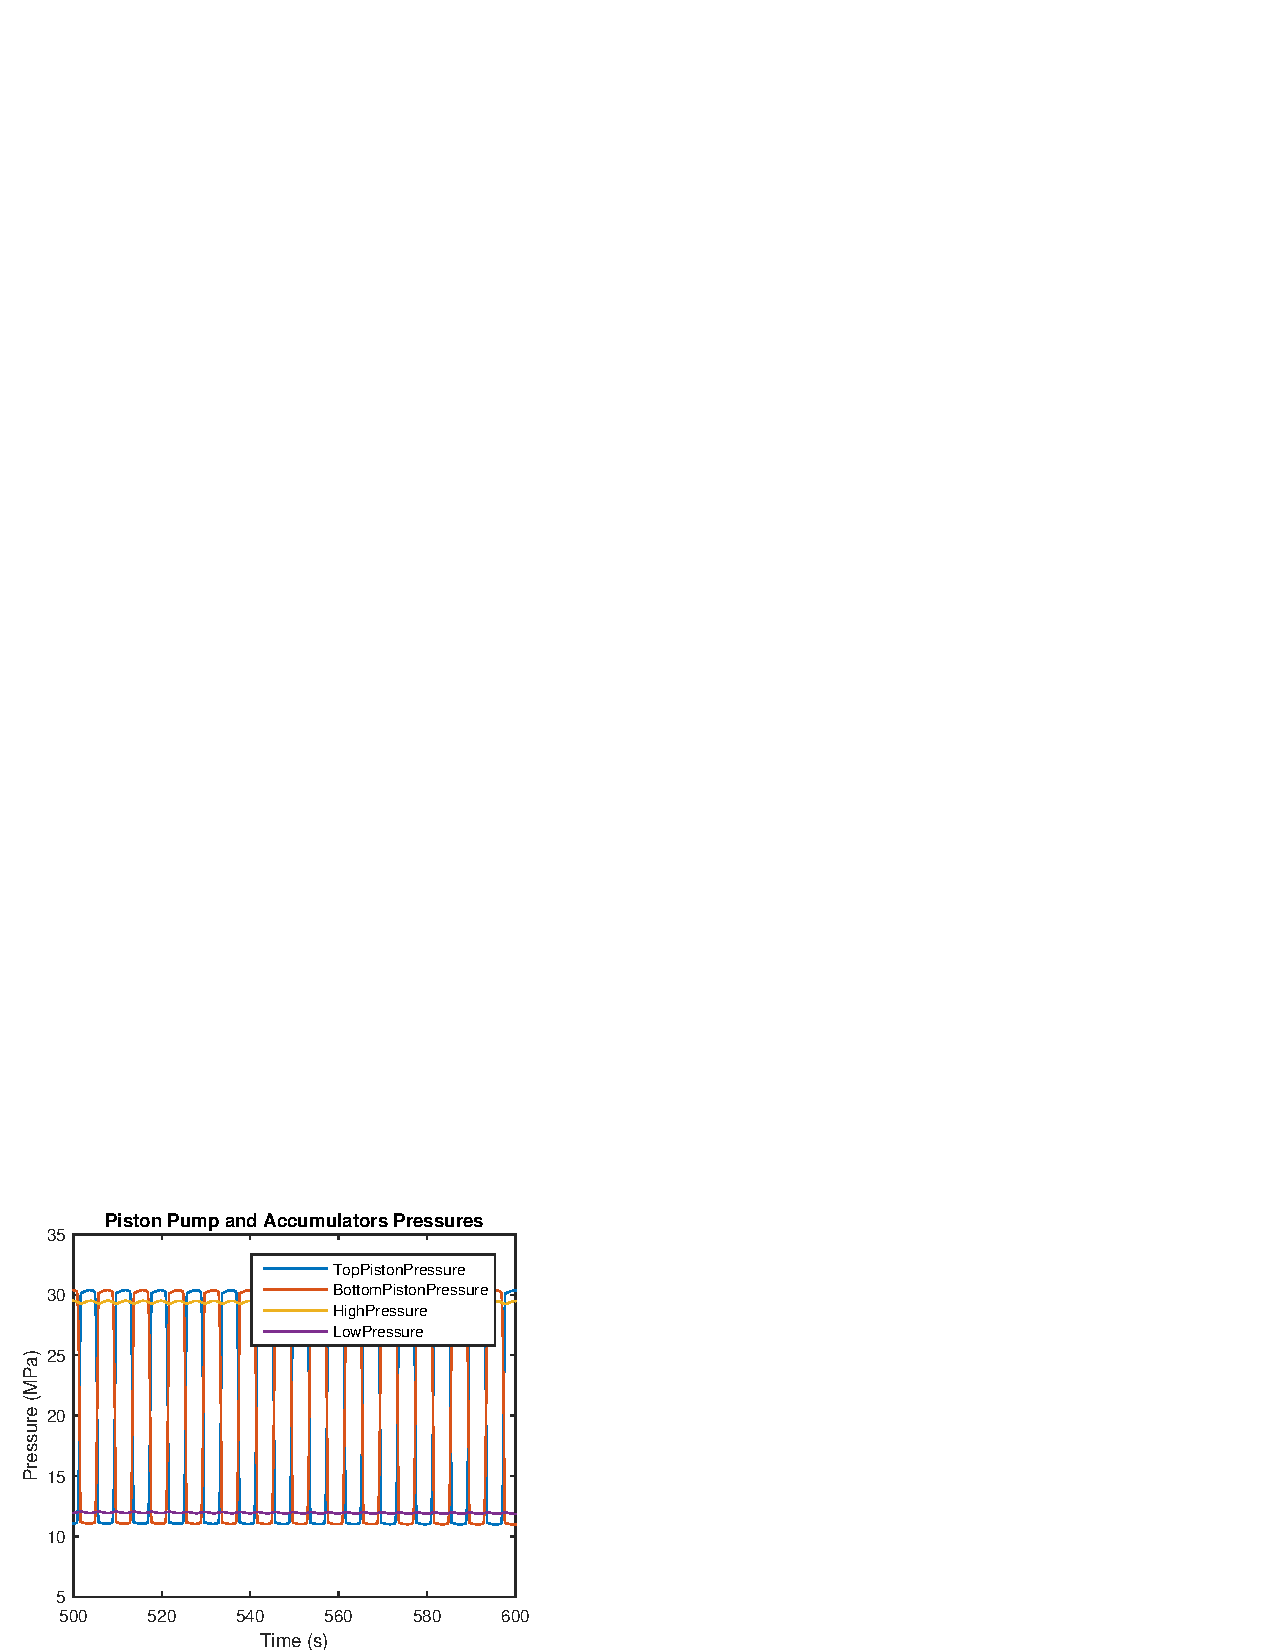
\includegraphics[width=1\columnwidth]{Images/Pressures}
    \caption{Piston pump and accumulators pressures. A check valve is open when either the top or bottom piston pressure is greater than the high pressure accumulator or less than the low pressure accumulator.}
    \label{HydPr}
    \end{figure}

\subsubsection*{Analysis.}    
   
 \begin{figure}[t]
     \centering
     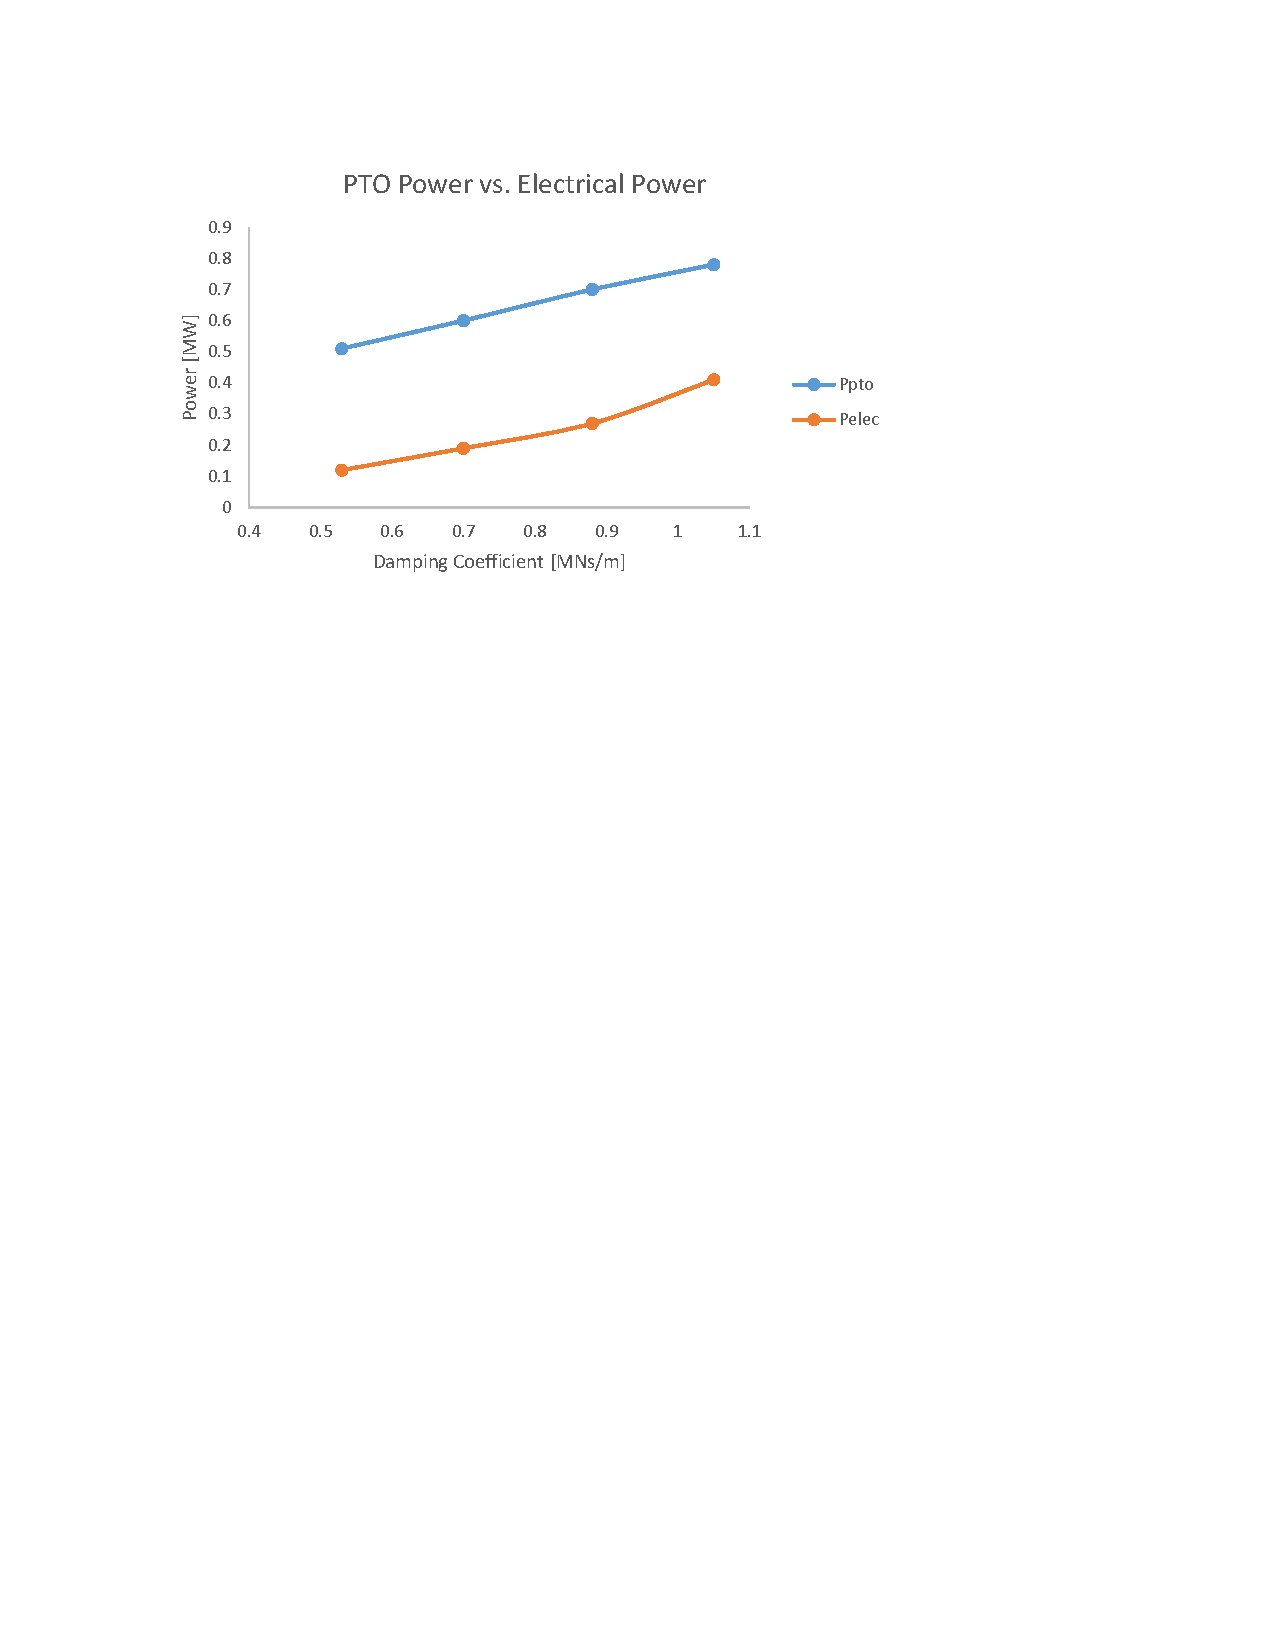
\includegraphics[width=1\columnwidth]{Images/PptovsPelec}
     \caption{A comparison between PTO power (WEC-Sim with constant damping) and electrical power (WEC-Sim with hydraulic PTO) when the dampings are the same. Damping coefficient is defined as the ratio of PTO force over relative heave velocity.}
     \label{HydDamping}
     \end{figure}  
   
 The plot shows in Fig.~\ref{HydDamping} compared an ideal PTO power against electrical power of the hydraulic PTO system at different damping coefficient. In ideal PTO case, the power is higher but it does not have a physical meaning. On the other hand, the electrical power from the hydraulic PTO system is lower but it represents the real meaning. 
 
    
%%%%%%%%%%%%%%%%%%%%%%%%%%%%%%%%%%%%%%%%%%%%%%%%%%%%%%%%%%%%%%%%%%%%%%
\subsection*{DIRECT DRIVE PTO}
Alternative to hydraulics, the direct drive power take off has less moving parts which allows a generator to capture power directly from the WEC movement. In this architecture, the PTO uses the direct buoy motion to drive the generator. The stator portion of the generator is contained in the WEC spar, while the buoy contains the magnets. This is illustrated in Fig.~\ref{L10}. The buoy movement causes the magnetic field surrounding the coils to change, the fundamental method for generating electricity. While this architecture has fewer power transformation stages and moving parts, it also has no inherent power storage capability (unlike the hydraulic system).

The direct drive approach can be constructed to deliver single or multiple-phase power by the arrangement of the generator magnets and coils. A three-phase winding was used in this model, enabling a valid comparison with the hydraulic model.  

The governing equation for a direct drive PTO is listed below. 
\begin{equation}
T_{em}=k(\lambda_{sd}i_{sq}- \lambda_{sq}i_{sd})
\end{equation}
\noindent where $k = P/2$ for rotational generator and $k = \pi/\tau_{pm}$ for a linear generator. $P$ is the number of poles ($P$ is greater or equal to 2, even number). $\tau_{pm}$ is the magnet pole pitch (the distance measured of the magnet from the center of one pole to the center of the next pole). The generator is modeled in the synchronous reference frame, where $\lambda_{sd}$ is the stator d-axis flux linkage, $i_{sq}$ is the stator q-axis current, $\lambda_{sq}$ is the stator q-axis flux linkage, and $i_{sd}$ is the stator d-axis current.  Derivation can be found in \cite{mohan2001advanced}.

Assuming the d-axis is aligned with the stator flux such that $\lambda_{sq} = 0$, Eq.(10) leads to Eq.(11), which describes the electromagnetic force for a linear electric machine. 
\begin{equation}
F_{em}=(\pi/\tau_{pm})\lambda_{sd}i_{sq}
\end{equation}

\begin{figure}[t]
    \centering
    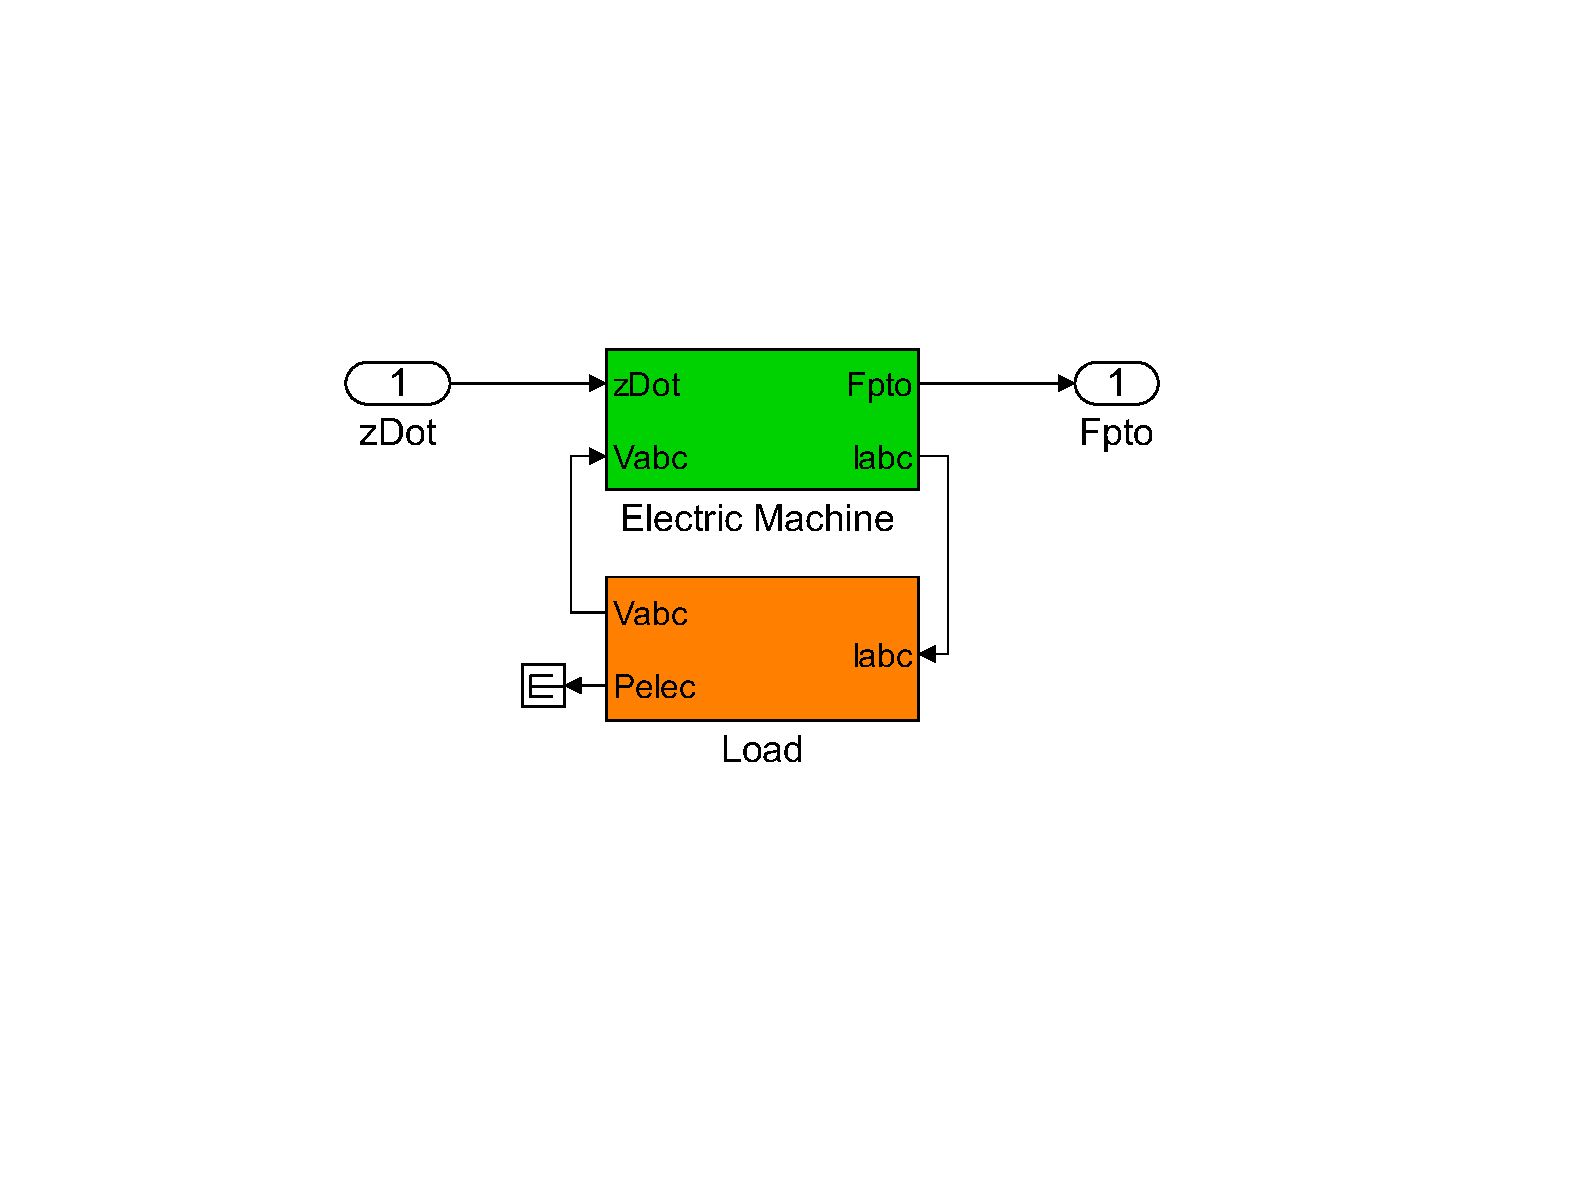
\includegraphics[width=1\columnwidth]{Images/DirectDriveSimulink}
    \caption{Schematic of the PTO-Sim direct drive model.}
    \label{DD}
    \end{figure}

The direct drive PTO model presented in this paper is based on \cite{prudell2009novel}. The generator stator consists of three-phase armature windings in 4 slots per phase for a total of 12 slots. There are always 2 pole pairs in the active region at any given time as shown in Fig.~\ref{magnets}.   

\begin{figure}[t]
    \centering
    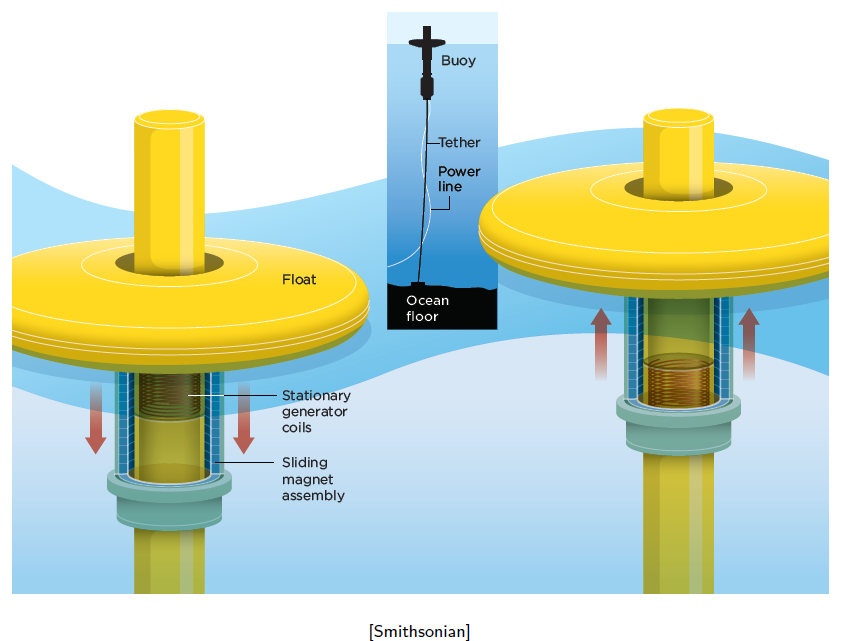
\includegraphics[width=1\columnwidth]{Images/PAWECSmithsonian}
    \caption{Direct Drive: OSU L10. This figure shows the stationary generator coils located inside the spar and the sliding magnet assembly coupled to the float.  (Image courtesy of Smithsonian Magazine) \cite{Rusch:2009aa}.} 
    \label{L10}
    \end{figure}

\begin{figure}[t]
    \centering
    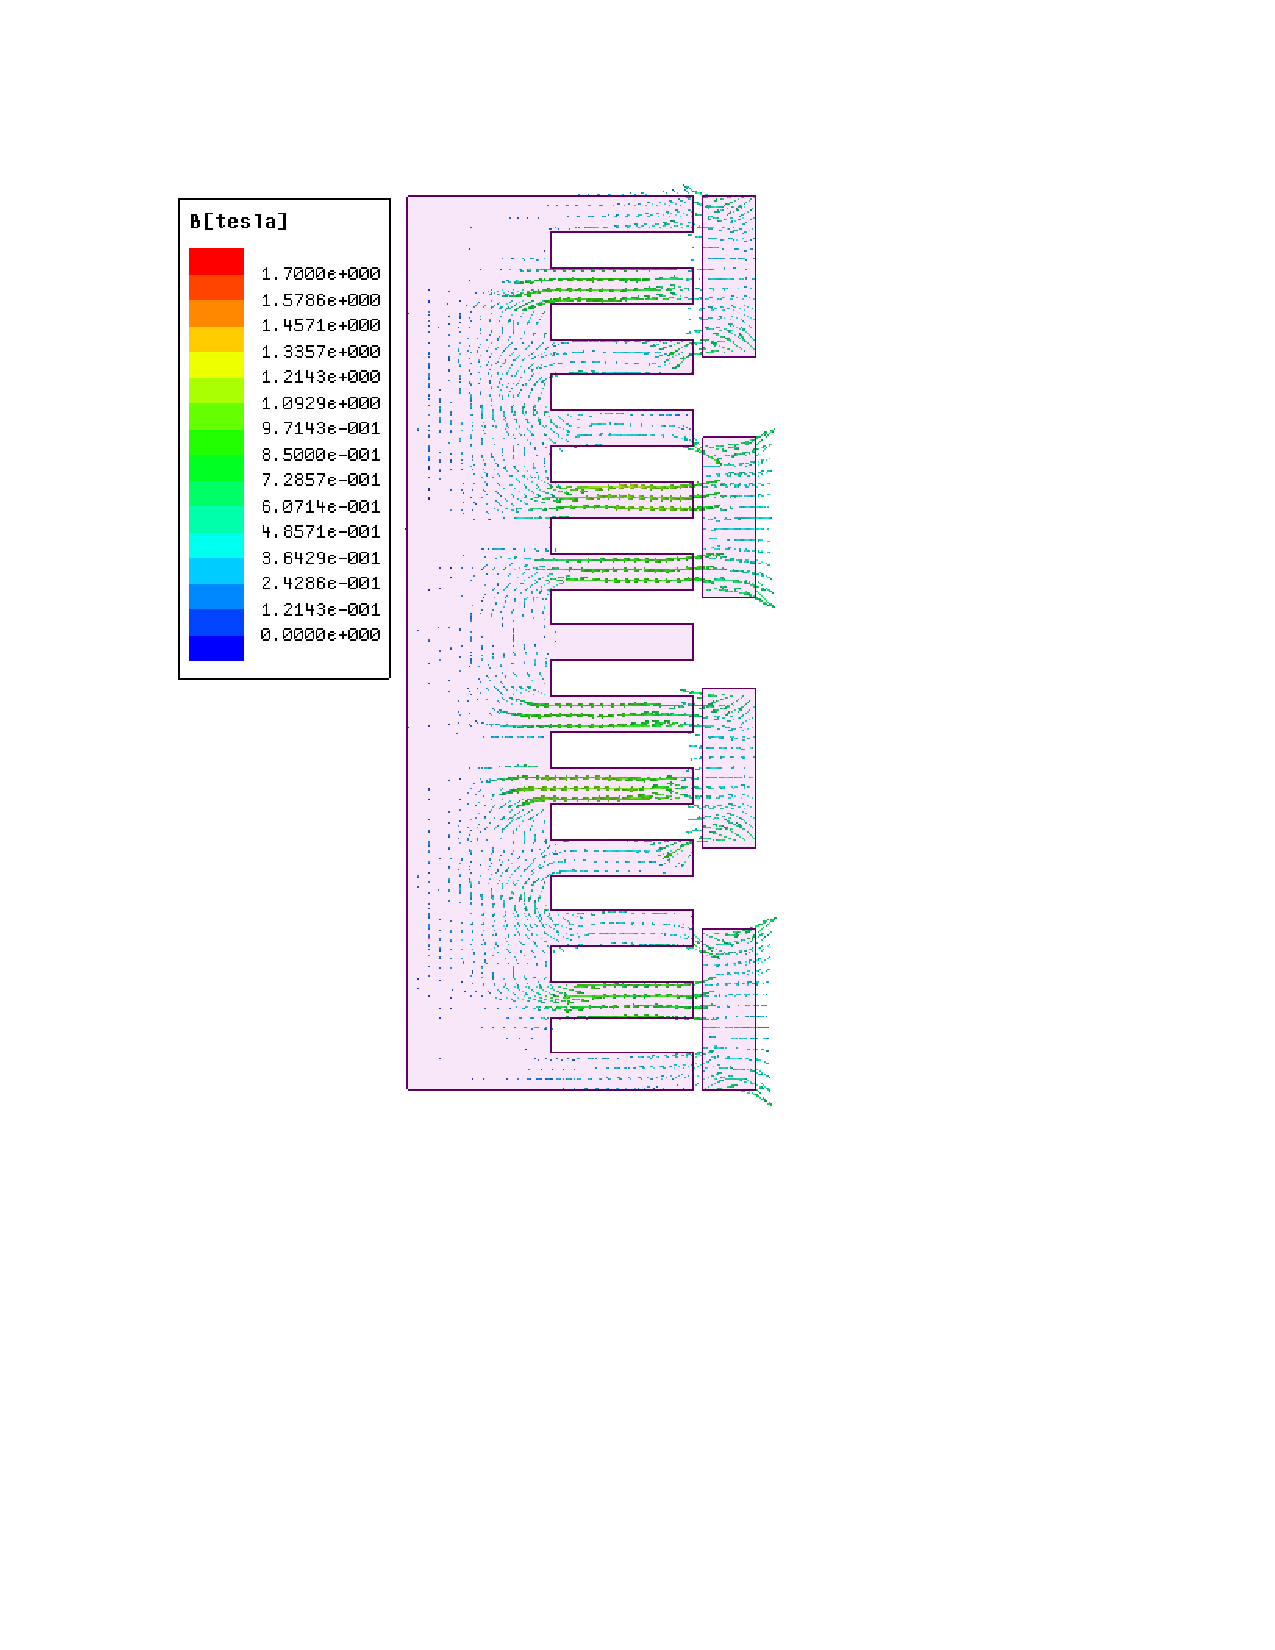
\includegraphics[width=1\columnwidth]{Images/Slots_n_Magnets_Linear}
    \caption{Cross section view of slots and magnets.}
    \label{magnets}
    \end{figure} 

The equivalent electrical circuit (Fig.~\ref{EMF}) shows the relationship between induced voltages $E_a, E_b,$ and $E_c$ and the external loads $R_{Load}$. $R_s$ and $L_s$ are the winding resistance and inductance of the coil. 

\begin{figure}[t]
    \centering
    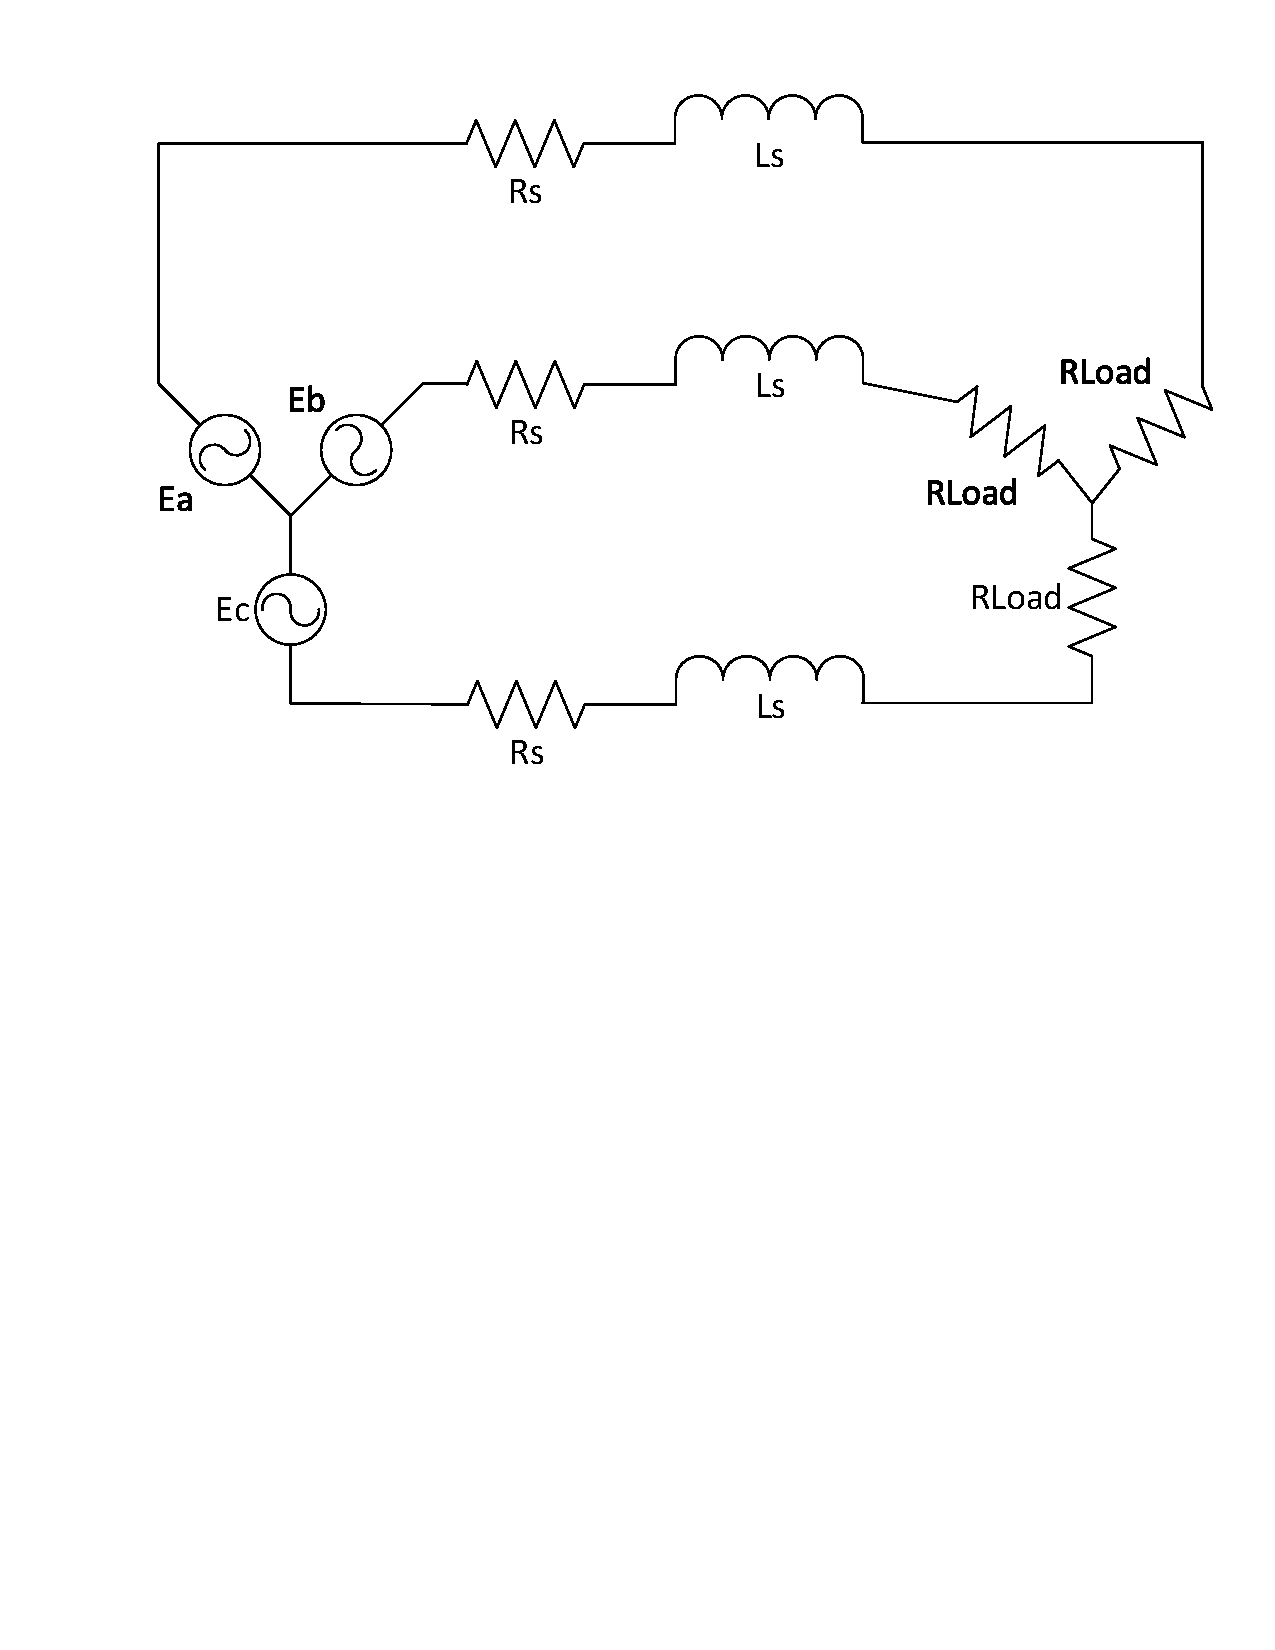
\includegraphics[width=1\columnwidth]{Images/BackEMFCkt}
    \caption{Back EMF circuit.}
    \label{EMF}
    \end{figure}

\subsubsection*{Simulations.}
 
The PTO was developed and verified with the use of regular waves. Once verified, irregular waves are applied, and the analysis can be focused on understanding the electrical power generated by the system. The same ``zDot" is used as an input for the direct drive PTO model as was used for the hydraulic PTO, see Fig.~\ref{HydZdot}. 

%Note (Kelley): The below statement is not true because zdot represents the relative motion between the float and the spar

%It is also assumed that the spar is stationary. 

%\begin{figure}[t]
%    \centering
%    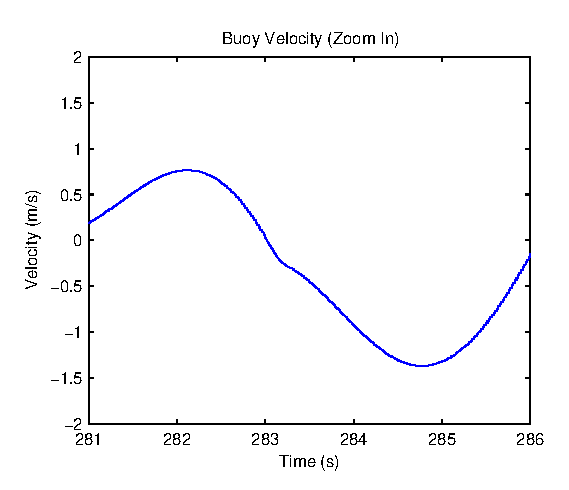
\includegraphics[width=1\columnwidth]{Images/DDzDotZoomIn}
%    \caption{The same buoy velocity but zoom in to show a time window between 281 and 286 seconds.}
%    %\label{fig-freq-comparison}
%    \end{figure}

The PTO force, shown in Fig.~\ref{DD_Fpto}, produced by the ``Electric Machine" model directly follows ``zDot" because of the nature of the direct drive design. Figures~\ref{voltage} and~\ref{current} show voltage and current in the external load. It should be noted that the magnitude of the voltage and current depends on the wave climate, and the WEC design parameters \cite{prudell2009novel}.  The absorbed and electric power are shown in Fig.~\ref{DDP}. 

\begin{figure}[t]
    \centering
    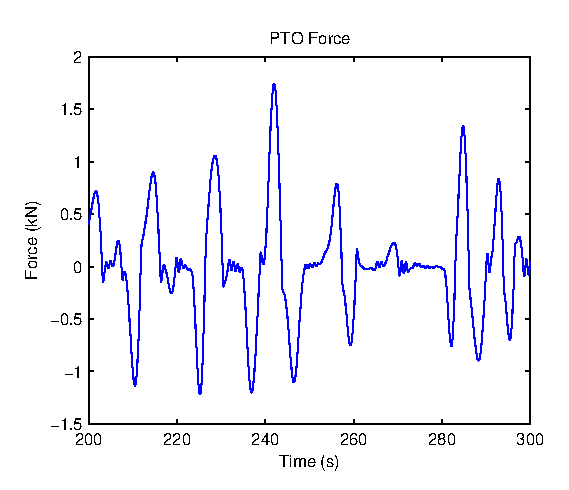
\includegraphics[width=1\columnwidth]{Images/DDFpto}
    \caption{Direct drive PTO force.}
    \label{DD_Fpto}
    \end{figure}

\begin{figure}[t]
    \centering
    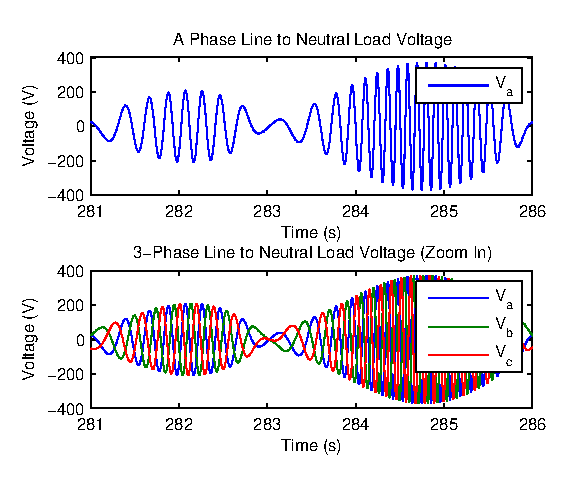
\includegraphics[width=1\columnwidth]{Images/DDVabc}
    \caption{Direct drive 3-phase line to neutral load voltage. As the PTO speed increases, both voltage magnitude and electric frequency increase.}
    \label{voltage}
    \end{figure}

\begin{figure}[t]
    \centering
    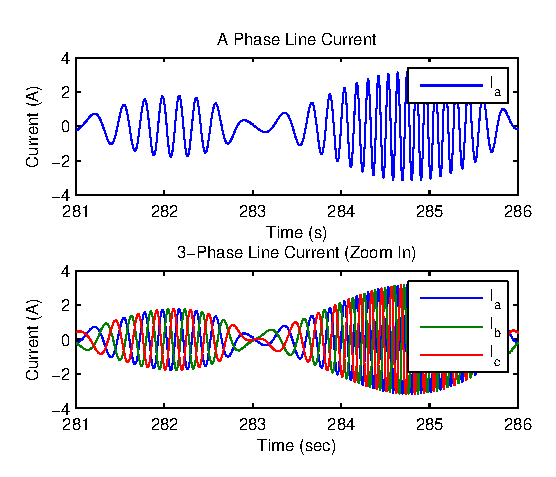
\includegraphics[width=1\columnwidth]{Images/DDIabcZoom}
    \caption{Direct drive 3-phase current.}
    \label{current}
    \end{figure}

\begin{figure}[t]
    \centering
    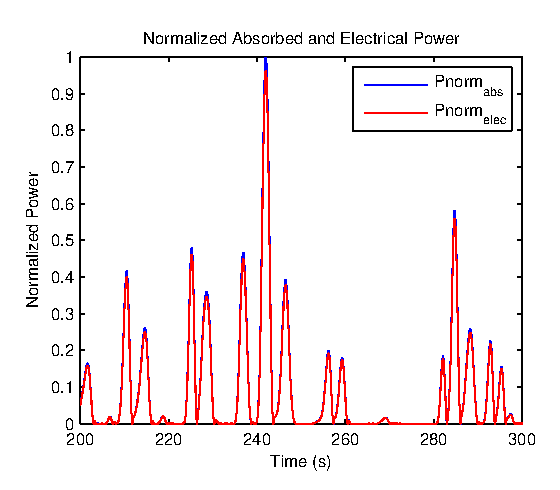
\includegraphics[width=1\columnwidth]{Images/normDDPabsPelec}
    \caption{Absorbed and Electrical Power. Efficiency is calculated to be about 96 \%.}
    \label{DDP}
    \end{figure}
    
    
%%%%%%%%%%%%%%%%%%%%%%%%%%%%%%%%%%%%%%%%%%%%%%%%%%%%%%%%%%%%%%%%%%%%%%
\subsection*{Generated Power Comparisons}

The usefulness of the PTO-Sim tool is exemplified by comparing the results from the two different architectures. The output electrical power for each PTO architecture are normalized and plotted in Fig.~\ref{Pnorm}. This figure clearly shows the native storage capability of the hydraulic system, which manifests as a smoother power profile. In contrast, the direct drive architecture power output is irregular, and a direct reflection of the incident sea state. 

\begin{figure}[t]
    \centering
    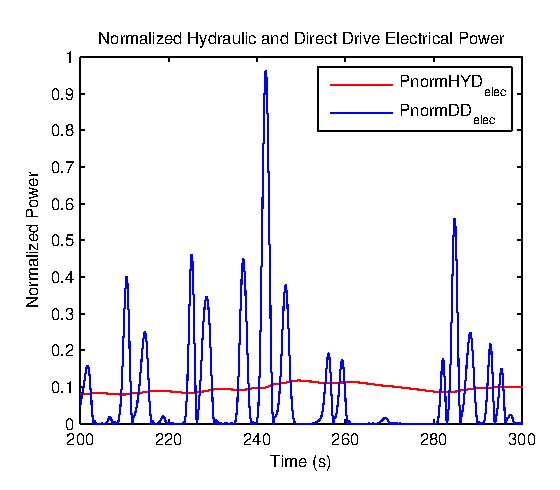
\includegraphics[width=1\columnwidth]{Images/HDYnDDelecPower}
    \caption{Comparison Between Normalized Hydraulic and Direct Drive Electrical Power.}
    \label{Pnorm}
    \end{figure}


 %%%%%%%%%%%%%%%%%%%%%%%%%%%%%%%%%%%%%%%%%%%%%%%%%%%%%%%%%%%%%%%%%%%%%
\section*{CONCLUSIONS}

This paper demonstrates the development and application of PTO-Sim, the WEC-Sim module responsible for accurately modeling WEC conversion of mechanical power to electrical power through its PTO system (or power conversion chain, PCC). While the initial release of WEC-Sim, Version 1.0, included the ability to model a WEC's PTO system as a simple linear damper, PTO-Sim allows users to model more complicated WEC PCCs. To demonstrate the functionality of PTO-Sim, two applications of PTO-Sim were shown in the paper, one of a hydraulic PTO system, and one of a direct drive PTO system. These two configurations were chosen because they reflect the two most common WEC PTO systems, for WECs of TRL 5+.  The demonstration results included illustrate the typical high-efficiencies of direct drive systems, but also illustrate the power smoothing (i.e., energy storage) inherent to hydraulic systems.  Once fully coupled with WEC-Sim, PTO-Sim will be released with future versions of the WEC-Sim code.


%%%%%%%%%%%%%%%%%%%%%%%%%%%%%%%%%%%%%%%%%%%%%%%%%%%%%%%%%%%%%%%%%%%%%%
\begin{acknowledgment}

This research was made possible by support from the Wind and Water Power Technologies Office within the DOE Office of Energy Efficiency \& Renewable Energy. The work was supported by Sandia National Laboratories and by the National Renewable Energy Laboratory. Sandia National Laboratories is a multi-program laboratory managed and operated by Sandia Corporation, a wholly owned subsidiary of Lockheed Martin Corporation, for the U.S. Department of Energy’s National Nuclear Security Administration under contract DE-AC04-94AL85000.

Figure 2 and 3 are contributed by Sam Kanner (University of California Berkeley) and figure 4 and 5 are contributed by Sean Casey (Energy Storage Systems, Inc.)

\end{acknowledgment}


%%%%%%%%%%%%%%%%%%%%%%%%%%%%%%%%%%%%%%%%%%%%%%%%%%%%%%%%%%%%%%%%%%%%%%
% bibliography

% Here's where you specify the bibliography style file.
% The full file name for the bibliography style file 
% used for an ASME paper is asmems4.bst.
\bibliographystyle{asmems4}
% Here's where you specify the bibliography database file.
% The full file name of the bibliography database for this
% article is asme2e.bib. The name for your database is up
% to you.
%\bibliography{asme2e}
\bibliography{ptosimbib}

%%%%%%%%%%%%%%%%%%%%%%%%%%%%%%%%%%%%%%%%%%%%%%%%%%%%%%%%%%%%%%%%%%%%%%
\end{document}



%%%%%%%%%%%%%%%%%%%%%%%%%asme2e.tex%%%%%%%%%%%%%
% Template for producing ASME-format articles using LaTeX            %
% Written by   Harry H. Cheng                                        %
%              Integration Engineering Laboratory                    %
%              Department of Mechanical and Aeronautical Engineering %
%              University of California                              %
%              Davis, CA 95616                                       %
%              Tel: (530) 752-5020 (office)                          %
%                   (530) 752-1028 (lab)                             %
%              Fax: (530) 752-4158                                   %
%              Email: hhcheng@ucdavis.edu                            %
%              WWW:   http://iel.ucdavis.edu/people/cheng.html       %
%              May 7, 1994                                           %
% Modified: February 16, 2001 by Harry H. Cheng                      %
% Modified: January  01, 2003 by Geoffrey R. Shiflett                %
% Use at your own risk, send complaints to /dev/null                 %
%%%%%%%%%%%%%%%%%%%%%%%%%%%%%%%%%%%%%%%%%%%



%%%%%%%%%%%%%%%%%%%%%%%%%%%%%%%%%%%%%%%%%%%%%%%%%%%%%%%%%%%%%%%%%%%%%%
% Table Example
%%%%%%%%%%%%%%%%%%%%%%%%%%%%%%%%%%%%%%%%%%%%%%%%%%%%%%%%%%%%%%%%%%%%%%

%\begin{table}[t]
%\caption{THE TABLE CAPTION USES CAPITAL LETTERS, TOO.}
%\begin{center}
%\label{table_ASME}
%\begin{tabular}{c l l}
%& & \\ % put some space after the caption
%\hline
%Example & Time & Cost \\
%\hline
%1 & 12.5 & \$1,000 \\
%2 & 24 & \$2,000 \\
%\hline
%\end{tabular}
%\end{center}
%\end{table}


%%%%%%%%%%%%%%%%%%%%%%%%%%%%%%%%%%%%%%%%%%%%%%%%%%%%%%%%%%%%%%%%%%%%%%
% Equation Example
%%%%%%%%%%%%%%%%%%%%%%%%%%%%%%%%%%%%%%%%%%%%%%%%%%%%%%%%%%%%%%%%%%%%%%

%\begin{equation}
%f(t) = \int_{0_+}^t F(t) dt + \frac{d g(t)}{d t}
%\label{eq_ASME}
%\end{equation}


%%%%%%%%%%%%%%%%%%%%%%%%%%%%%%%%%%%%%%%%%%%%%%%%%%%%%%%%%%%%%%%%%%%%%%
% SubSection Example
%%%%%%%%%%%%%%%%%%%%%%%%%%%%%%%%%%%%%%%%%%%%%%%%%%%%%%%%%%%%%%%%%%%%%%

%\subsection*{Second-Level Heading}


%%%%%%%%%%%%%%%%%%%%%%%%%%%%%%%%%%%%%%%%%%%%%%%%%%%%%%%%%%%%%%%%%%%%%%
% SubSubSection Example
%%%%%%%%%%%%%%%%%%%%%%%%%%%%%%%%%%%%%%%%%%%%%%%%%%%%%%%%%%%%%%%%%%%%%%

%\subsubsection*{Third-Level Heading.}


